\documentclass[english,11pt,usenames,dvipsnames]{beamer}

\DeclareMathOperator{\Cov}{Cov}
\DeclareMathOperator{\Var}{Var}
\DeclareMathOperator{\E}{\mathbb{E}}
\DeclareMathOperator{\Proba}{\mathbb{P}}

\newcommand{\Covb}[2]{\ensuremath{\Cov\!\left[#1,#2\right]}}
\newcommand{\Eb}[1]{\ensuremath{\E\!\left[#1\right]}}
\newcommand{\Pb}[1]{\ensuremath{\Proba\!\left[#1\right]}}
\newcommand{\Varb}[1]{\ensuremath{\Var\!\left[#1\right]}}

% norm
\newcommand{\norm}[1]{\| #1 \|}

\newcommand{\indep}{\rotatebox[origin=c]{90}{$\models$}}





\usepackage{mathptmx,amsmath,amssymb,graphicx,bibentry,bbm,babel,ragged2e}

\makeatletter

\newcommand{\noun}[1]{\textsc{#1}}
\newcommand{\jitem}[1]{\item \begin{justify} #1 \end{justify} \vfill{}}
\newcommand{\sframe}[2]{\frame{\frametitle{#1} #2}}

\newenvironment{centercolumns}{\begin{columns}[c]}{\end{columns}}
%\newenvironment{jitem}{\begin{justify}\begin{itemize}}{\end{itemize}\end{justify}}

\usetheme{Warsaw}
\setbeamertemplate{footline}[text line]{}
\setbeamercolor{structure}{fg=purple!50!blue, bg=purple!50!blue}

\setbeamersize{text margin left=15pt,text margin right=15pt}

\setbeamercovered{transparent}

\setbeamertemplate{headline}{}
\setbeamertemplate{footline}[frame number]
\setbeamertemplate{navigation symbols}{}

\@ifundefined{showcaptionsetup}{}{%
 \PassOptionsToPackage{caption=false}{subfig}}
\usepackage{subfig}

\usepackage[utf8]{inputenc}
\usepackage[T1]{fontenc}


\usepackage{tikz}

\usepackage{multirow}


\usepackage{mdframed}

\usepackage[usenames,dvipsnames]{pstricks}
\usepackage{auto-pst-pdf}


\usepackage[dvipsnames]{xcolor}


\makeatother

\begin{document}


\title{Towards multi-scalar models for the co-evolution of transportation networks and territories}

\author{J.~Raimbault$^{1,2,3}$\\
\texttt{juste.raimbault@iscpif.fr}
}


\institute{$^{1}$UPS CNRS 3611 ISC-PIF\\
$^{2}$CASA, UCL\\
$^{3}$UMR CNRS 8504 G{\'e}ographie-cit{\'e}s
}


\date{Theo Quant 2019\\\smallskip
6 février 2019
}

\frame{\maketitle}

% Keywords: Transportation networks; Territories; Co-evolution; Modeling; Multi-scale

% plan :
%   - co-evolution : difficult issues
%   - recall previous results
%   - describe model with physical nw (heuristic, synthetic setup etc)
%.  - perspective : describe multi-scalar avec mesocoevol (two entries into multiscalar : "top-down" (precise a macro model) ; "bottom-up" (inserting meso instances into a macro coupling structure.



\section{Introduction}


\sframe{Interactions between networks and territories}{

%The intricate relations between transportation networks and territories, at multiples scales, has fed numerous open questions such as the potential existence of structuring effects of networks \cite{offner1993effets}.

% striking example for Besac.

Central role of interactions between networks and territories in urban systems dynamics

\medskip

\centering

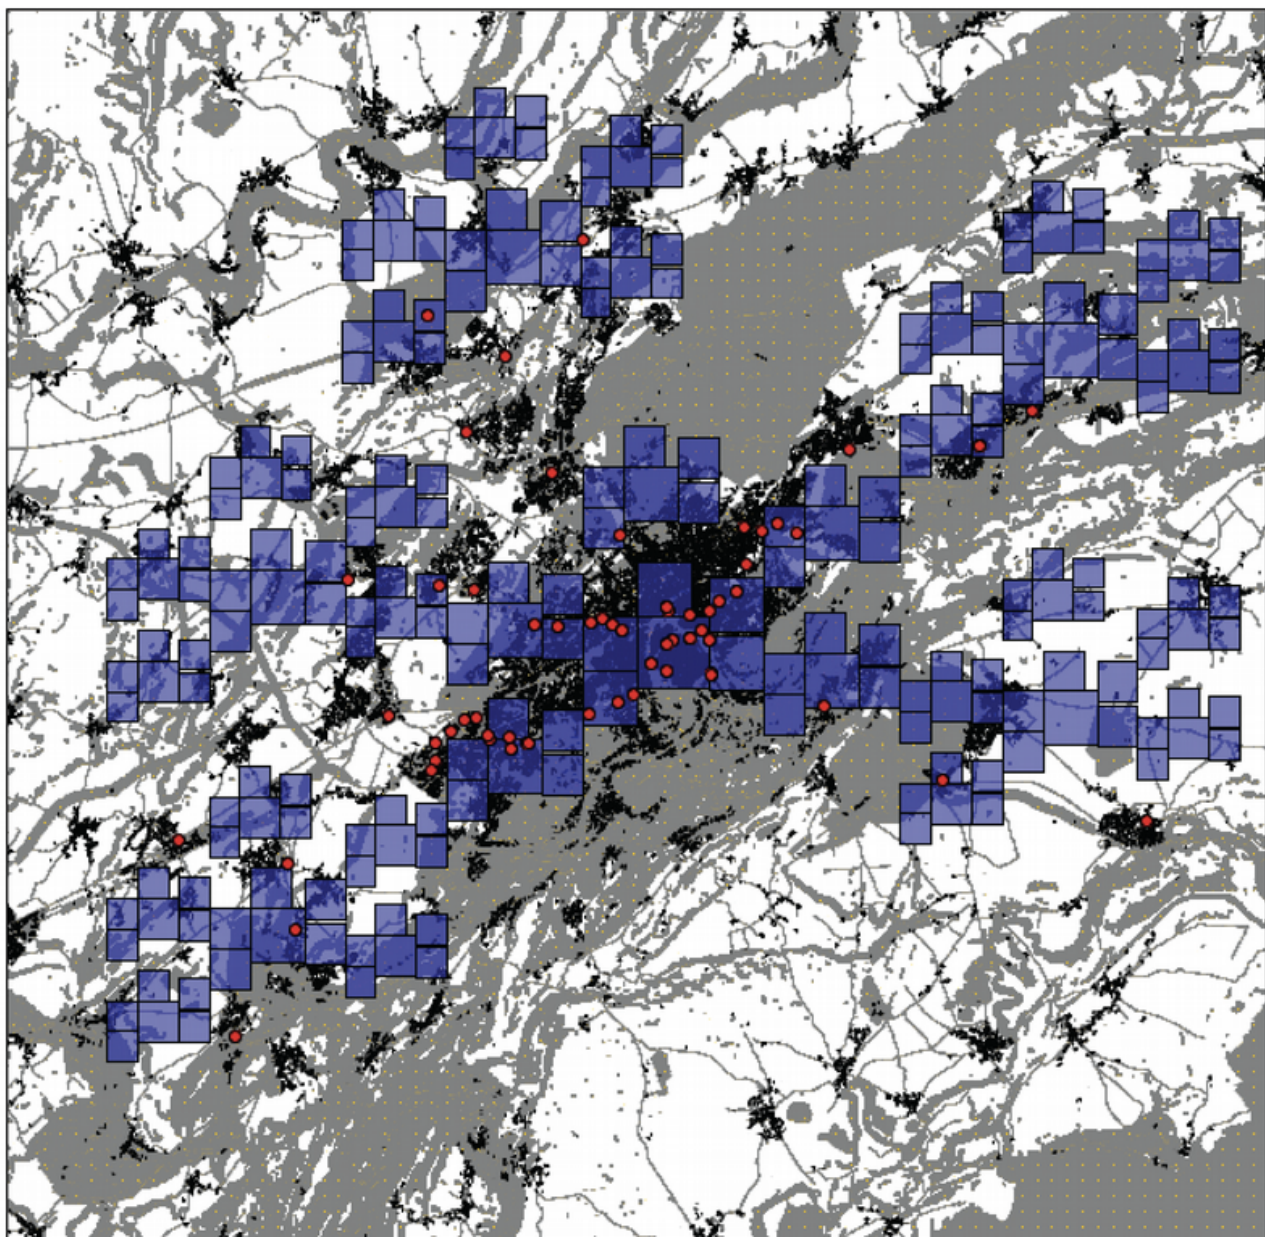
\includegraphics[height=0.75\textheight]{figures/fractalopolis.png}

\footnotesize

\textit{Example: Multifractal planning for the city of Besancon \cite{tannier:tel-01668615}}


}



\sframe{Modeling the co-evolution of networks and territories}{
 
 % \cite{raimbault2018caracterisation} explored these interactions from the point of view of co-evolutive dynamics, aiming at modeling these. In particular, \cite{raimbault2018modeling} introduced a co-evolution model at the macroscopic scale for systems of cities with abstract networks, whereas \cite{raimbault2018urban} developed a morphogenesis model at the mesoscopic scale, capturing the co-evolution between road networks and the population density grid.
 
 \vspace{-1cm}
\textit{Models with different ontologies and scales \cite{raimbault2018caracterisation}}

\bigskip
\bigskip

%\setlength{\columnseprule}{0.4pt}

\begin{columns}
\begin{column}{0.50\textwidth}
\centering\textbf{Macroscopic}
\end{column}
%\vrule{}
%\vrule{}
\begin{column}{0.50\textwidth}
\centering\textbf{Mesoscopic}
\end{column}
\end{columns}

\bigskip

\begin{columns}
\begin{column}{0.4\textwidth}
\centering
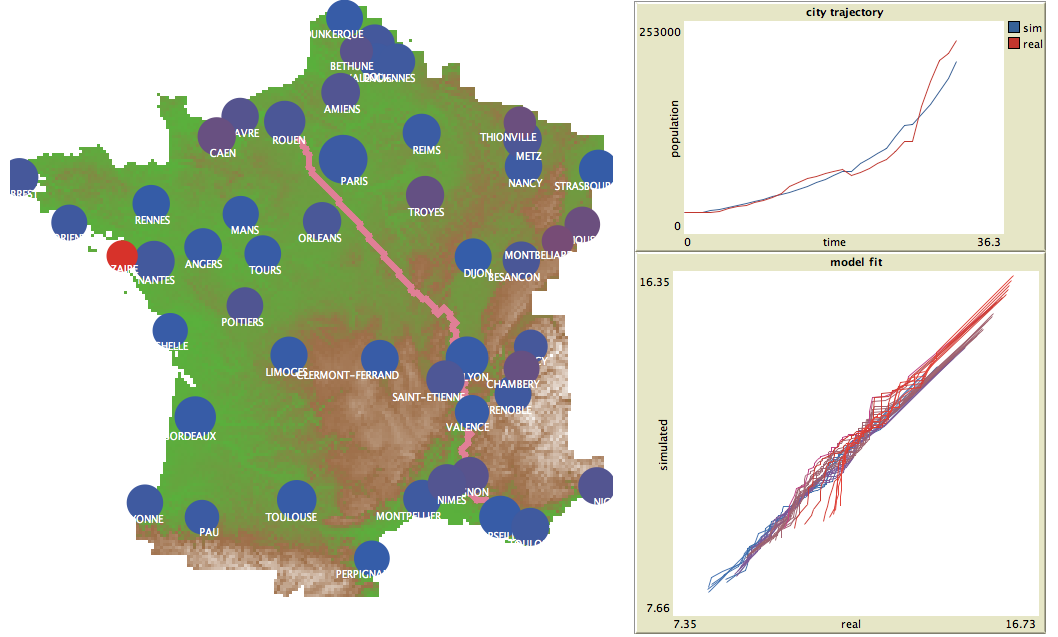
\includegraphics[width=\textwidth]{figures/intgib_Fig2.png}

\bigskip

\footnotesize\textit{Interaction model}



\end{column}

\vspace*{-1cm}\vrule{}
\begin{column}{0.35\textwidth}

\centering

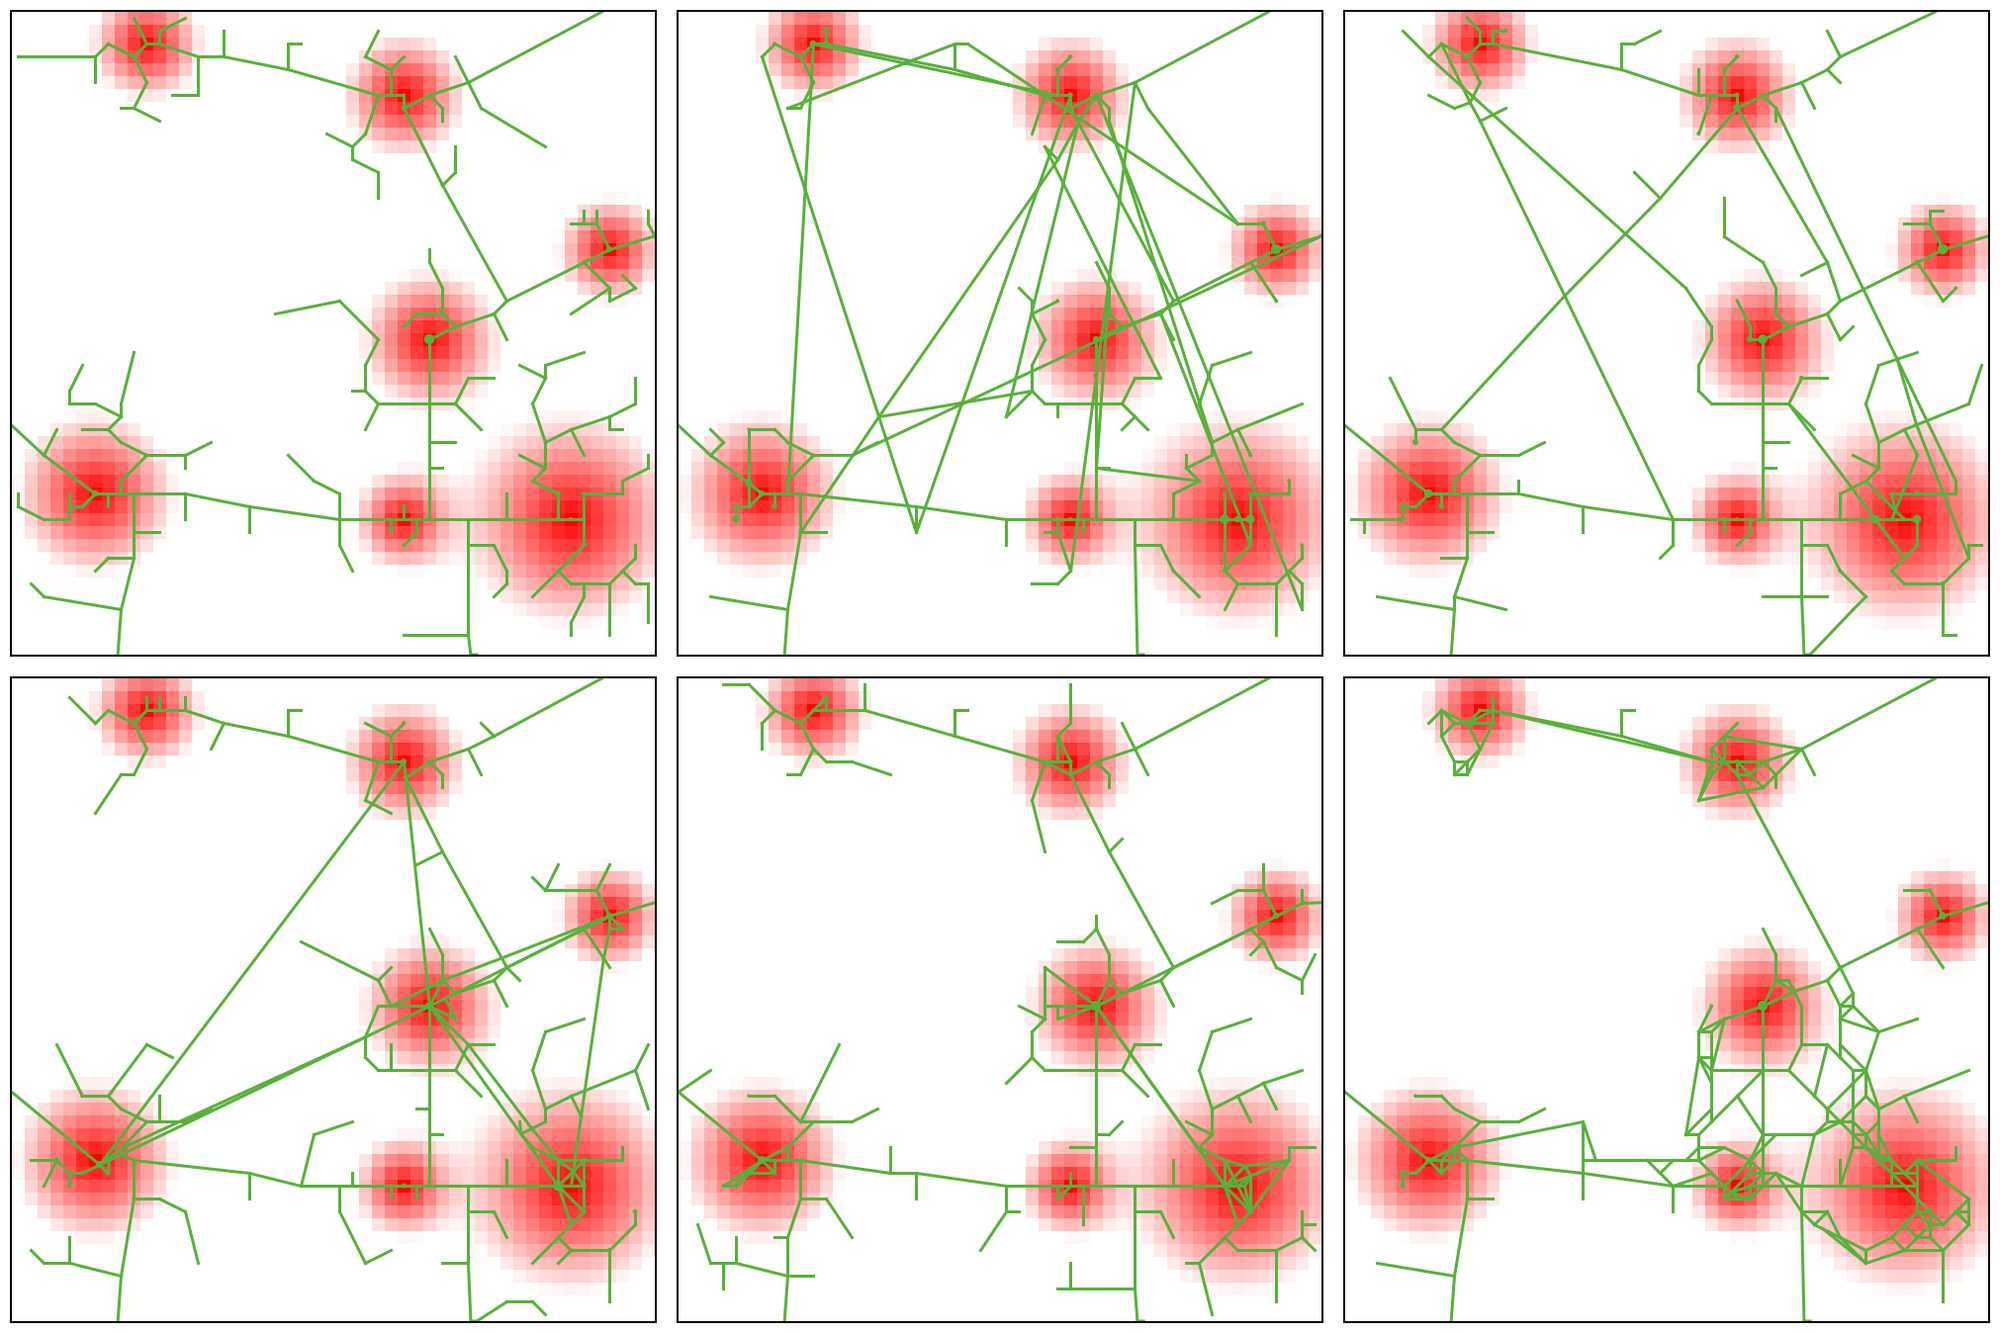
\includegraphics[width=\columnwidth]{figures/7-1-2-fig-networkgrowth-examples.jpg}

\bigskip

\footnotesize\textit{Urban morphogenesis}
%
\end{column}

%\vrule{}
%\begin{column}{0.25\textwidth}
%\centering
%\includegraphics[width=\textwidth]{figuresraw/coevol_example_nw-cost}\\
%\footnotesize\textit{Co-evolution model}
%\medskip
%\it\textbf{Explication}
%\end{column}

\vrule{}
\begin{column}{0.2\textwidth}
\centering
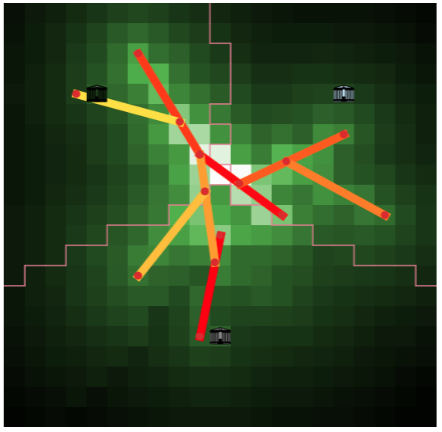
\includegraphics[width=\textwidth]{figures/lutetia_longtimelimit_2.png}\\

\bigskip

\footnotesize\textit{Transportation governance}

\end{column}
\end{columns}


  
 
}



\sframe{Towards multi-scalar models}{

% The processes included in models depend naturally on the scale. This communication aims at showing the necessity of a multi-scalar approach for a more accurate account of these co-evolutive dynamics.

\justify


$\rightarrow$ Processes included depend on the scale (urban form and function, interactions between cities)

\bigskip

$\rightarrow$ Truly multi-scale models (coupling different ontologies and not just geographical ranges, and with a strong coupling between scales) are very rare (inexistent ?), despite a strong need for these \cite{rozenblat2018conclusion}

\bigskip
\bigskip

\textbf{Research objective: } \textit{Investigate an hybrid co-evolution model coupling macroscopic city dynamics and mescoscopic network dynamics}


}


\sframe{Generic description of the model}{

% We introduce first a physical implementation of transportation networks into the macroscopic model, with a description of networks with a 1km spatial resolution, whereas the typical range of application of the model is around 1000km.



\centering

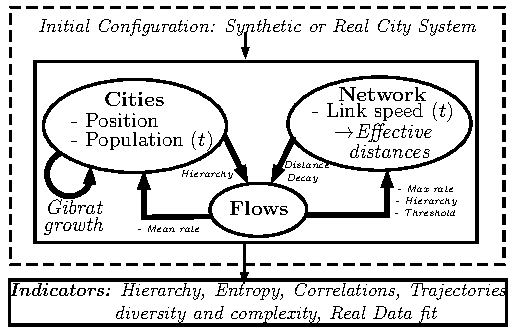
\includegraphics[width=\textwidth]{figures/model.pdf}

}

\sframe{Macroscopic interaction model}{

\begin{pspicture}(0,-2.91)(11.46,2.91)
\definecolor{colour0}{rgb}{0.2,0.6,0.0}
\definecolor{colour1}{rgb}{1.0,0.0,0.2}
\definecolor{colour2}{rgb}{0.0,0.4,0.8}
\pscircle[linecolor=black, linewidth=0.04, dimen=outer](0.8,0.29){0.8}
\pscircle[linecolor=black, linewidth=0.04, dimen=outer](3.44,-1.87){0.38}
\pscircle[linecolor=black, linewidth=0.04, dimen=outer](4.64,2.11){0.5}
\pscircle[linecolor=black, linewidth=0.04, dimen=outer](6.72,-2.09){0.48}
\rput[bl](0.28,0.39){\textit{City 1}}
\rput[bl](4.16,2.67){\textit{City 2}}
\rput[bl](2.88,-2.63){\textit{City 3}}
\rput[bl](6.16,-2.91){\textit{City 4}}
\pscircle[linecolor=black, linewidth=0.04, dimen=outer](7.56,2.49){0.44}
\pscircle[linecolor=black, linewidth=0.04, dimen=outer](7.56,2.39){0.34}
\pscircle[linecolor=black, linewidth=0.04, dimen=outer](7.56,2.29){0.22}
\rput[bl](8.18,2.19){Population}
\only<2->{
\psline[linecolor=black, linewidth=0.04, linestyle=dashed, dash=0.17638889cm 0.10583334cm](1.52,-0.11)(3.56,-1.27)(6.24,-1.99)
\psline[linecolor=black, linewidth=0.04, linestyle=dashed, dash=0.17638889cm 0.10583334cm](1.5,0.65)(4.14,1.89)
\psline[linecolor=black, linewidth=0.04, linestyle=dashed, dash=0.17638889cm 0.10583334cm](4.86,1.67)(6.42,-1.67)
\psline[linecolor=black, linewidth=0.04, linestyle=dashed, dash=0.17638889cm 0.10583334cm](3.54,-1.49)(4.46,1.65)
}
\only<3->{
\rput{-26.454165}(-0.3952402,0.39846048){\psarc[linecolor=colour0, linewidth=0.04, dimen=outer, arrowsize=0.05291667cm 2.0,arrowlength=1.4,arrowinset=0.0]{<-}(0.65,1.04){0.34}{25.401218}{227.9924}}
\psarc[linecolor=colour0, linewidth=0.04, dimen=outer, arrowsize=0.05291667cm 2.0,arrowlength=1.4,arrowinset=0.0]{<-}(4.08,2.13){0.28}{63.434948}{284.03625}
\psarc[linecolor=colour0, linewidth=0.04, dimen=outer, arrowsize=0.05291667cm 2.0,arrowlength=1.4,arrowinset=0.0]{<-}(3.0,-1.91){0.24}{54.162346}{315.0}
\rput{132.8386}(10.745382,-8.510234){\psarc[linecolor=colour0, linewidth=0.04, dimen=outer, arrowsize=0.05291667cm 2.0,arrowlength=1.4,arrowinset=0.0]{<-}(7.23,-1.91){0.41}{126.483}{346.42313}}
\psline[linecolor=colour0, linewidth=0.04, arrowsize=0.05291667cm 2.0,arrowlength=1.4,arrowinset=0.0]{<-}(7.18,1.83)(8.0,1.83)
\rput[bl](8.16,1.69){Endogenous growth}
}
\only<4->{
\psline[linecolor=colour0, linewidth=0.08, arrowsize=0.05291667cm 2.0,arrowlength=1.4,arrowinset=0.0]{<->}(1.56,0.53)(4.18,1.77)
\psline[linecolor=colour0, linewidth=0.16, arrowsize=0.05291667cm 2.0,arrowlength=1.4,arrowinset=0.0]{<->}(1.6,0.07)(6.2,-1.85)
\psline[linecolor=colour0, linewidth=0.08, arrowsize=0.05291667cm 2.0,arrowlength=1.4,arrowinset=0.0]{<->}(4.8,1.53)(6.26,-1.73)
\psline[linecolor=colour0, linewidth=0.04, arrowsize=0.05291667cm 2.0,arrowlength=1.4,arrowinset=0.0]{<->}(1.44,-0.29)(3.16,-1.51)
\psline[linecolor=colour0, linewidth=0.04, arrowsize=0.05291667cm 2.0,arrowlength=1.4,arrowinset=0.0]{<->}(3.86,-1.91)(6.2,-2.19)
\psline[linecolor=colour0, linewidth=0.04, arrowsize=0.05291667cm 2.0,arrowlength=1.4,arrowinset=0.0]{<->}(7.18,1.37)(8.08,1.37)
\rput[bl](8.2,1.29){Direct interaction}
}
\only<5->{
\psline[linecolor=colour1, linewidth=0.04, arrowsize=0.05291667cm 2.0,arrowlength=1.4,arrowinset=0.0]{<-}(3.38,-1.47)(3.56,-0.83)
\psline[linecolor=colour1, linewidth=0.04, arrowsize=0.05291667cm 2.0,arrowlength=1.4,arrowinset=0.0]{<-}(7.239434,0.8681779)(7.940566,0.8718221)
\rput[bl](8.16,0.79){Feedback of flows}
}
\only<6->{
\psarc[linecolor=colour2, linewidth=0.08, dimen=outer, arrowsize=0.05291667cm 2.0,arrowlength=1.4,arrowinset=0.0]{<-}(2.53,1.08){0.49}{31.297699}{206.56505}
\rput{24.443954}(0.36267212,-1.6543155){\psarc[linecolor=colour2, linewidth=0.08, dimen=outer, arrowsize=0.05291667cm 2.0,arrowlength=1.4,arrowinset=0.0]{<-}(4.0,0.01){0.3}{43.264294}{270.0}}
\rput{-24.545204}(0.48092335,2.1707923){\psarc[linecolor=colour2, linewidth=0.08, dimen=outer, arrowsize=0.05291667cm 2.0,arrowlength=1.4,arrowinset=0.0]{<-}(5.23,-0.02){0.73}{113.76878}{353.57126}}
\rput{-120.28376}(7.6030025,2.224528){\psarc[linecolor=colour2, linewidth=0.08, dimen=outer, arrowsize=0.05291667cm 2.0,arrowlength=1.4,arrowinset=0.0]{<-}(4.44,-1.07){0.46}{36.341637}{274.27374}}
\rput{-76.46916}(2.4050338,2.3124602){\psarc[linecolor=colour2, linewidth=0.08, dimen=outer, arrowsize=0.05291667cm 2.0,arrowlength=1.4,arrowinset=0.0]{->}(2.67,-0.37){0.4}{229.21208}{350.33667}}
\psline[linecolor=colour2, linewidth=0.04, arrowsize=0.05291667cm 2.0,arrowlength=1.4,arrowinset=0.0]{<-}(7.26,0.37)(7.96,0.37)
\rput[bl](8.14,0.25){Network adaptation}
}
\end{pspicture}


}





%\sframe{Physical network specification}{
%}


\sframe{Synthetic physical network}{

\textbf{Making the model hybrid: } physical network specification with explicit topology and geographical distribution; link capacity evolution with self-reinforcement

\bigskip

\centering

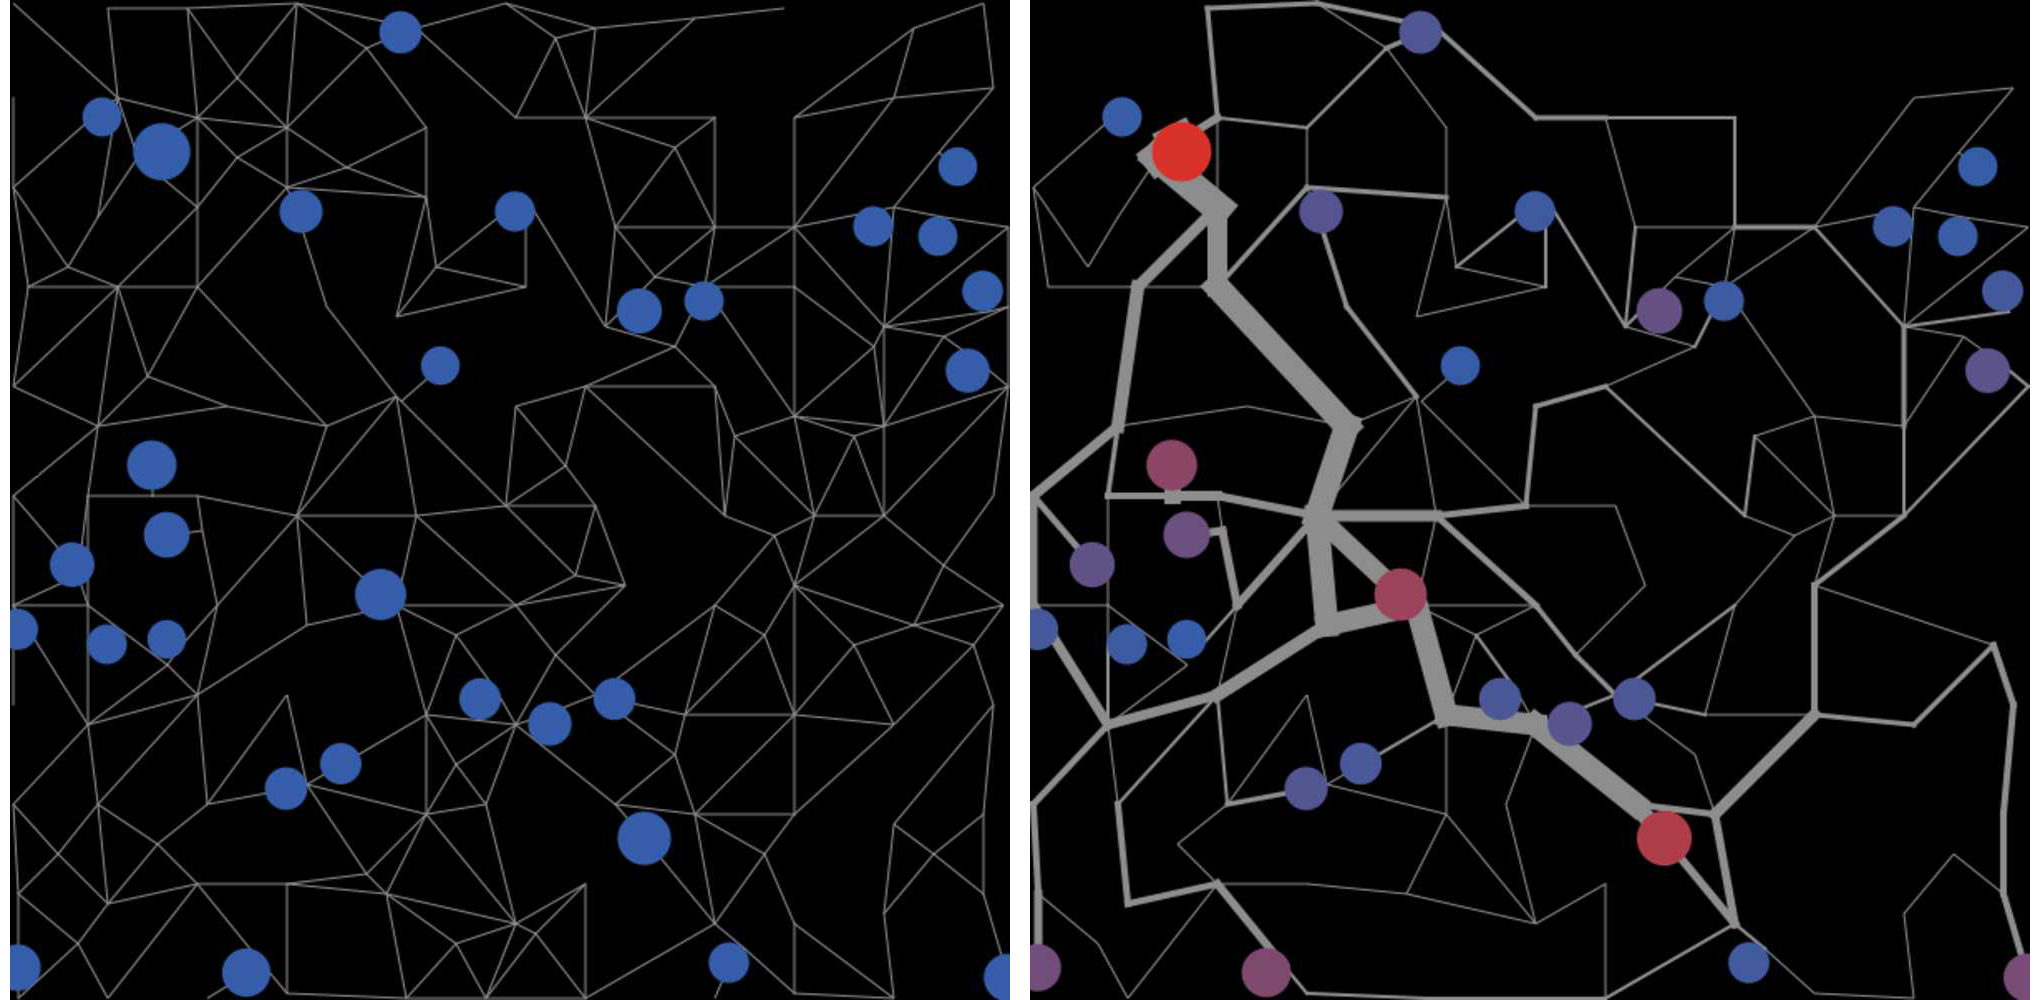
\includegraphics[width=0.8\textwidth]{figures/6-2-3-fig-macrocoevol-slimemould.jpg}

\medskip

\footnotesize \textit{Illustration on a synthetic system of cities}

}

\sframe{Real physical network}{
% Railway network

\textit{Parametrisation on the French system of cities with temporal windows (see \cite{raimbault2018indirect}); train network data from \cite{mimeur:hal-01616746}}


\bigskip


\centering

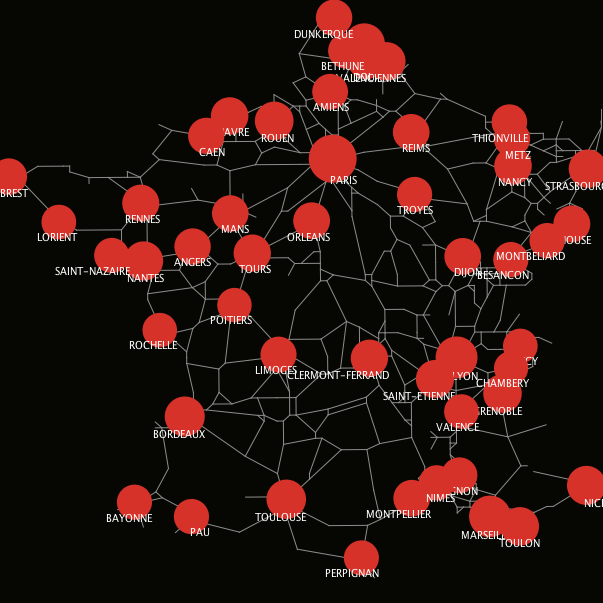
\includegraphics[width=0.48\textwidth]{figures/ex_real_1975.png}\hspace{0.1cm}
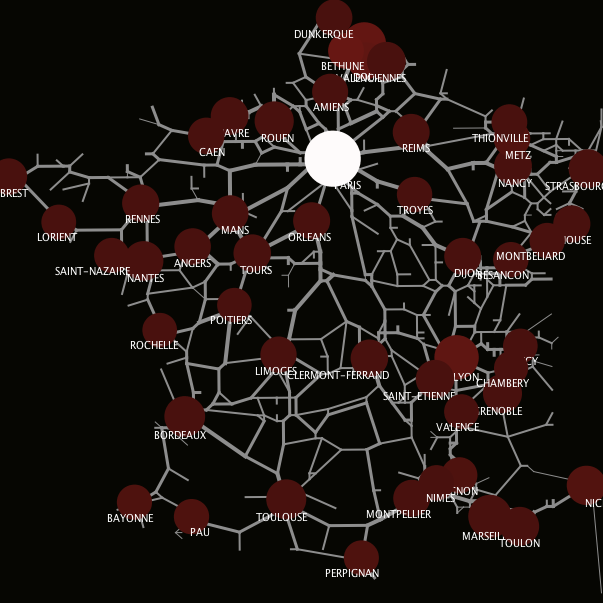
\includegraphics[width=0.48\textwidth]{figures/ex_real_1975_tf_adjusted.png}

}






\sframe{Model exploration and calibration}{

% Calibrations are done for different versions of each model including more or less parameters, using distributed genetic algorithms on a computation grid through the intermediary of the OpenMOLE model exploration software [6]. 

Large experience plan and bi-objective calibration on 9 periods $\rightarrow$ use of genetic algorithms on grid, made smooth with the OpenMOLE software \url{https://next.openmole.org/}

\centering

\smallskip


\includegraphics[height=0.35\textheight]{figures/openmole.png}

\smallskip

\raggedright\justify

\footnotesize \textit{OpenMOLE: (i) embed any model as a black box; (ii) transparent access to main High Performance Computing environments; (iii) model exploration and calibration methods.}

\bigskip

\textbf{Come to the demonstration tomorrow, and save the date for the next summer school (2020) !} 
\texttt{https://exmodelo.org/}

}



\sframe{Model behavior}{

\textit{Qualitatively similar trajectories in time}

\bigskip


\begin{columns}
	\begin{column}{0.45\linewidth}
		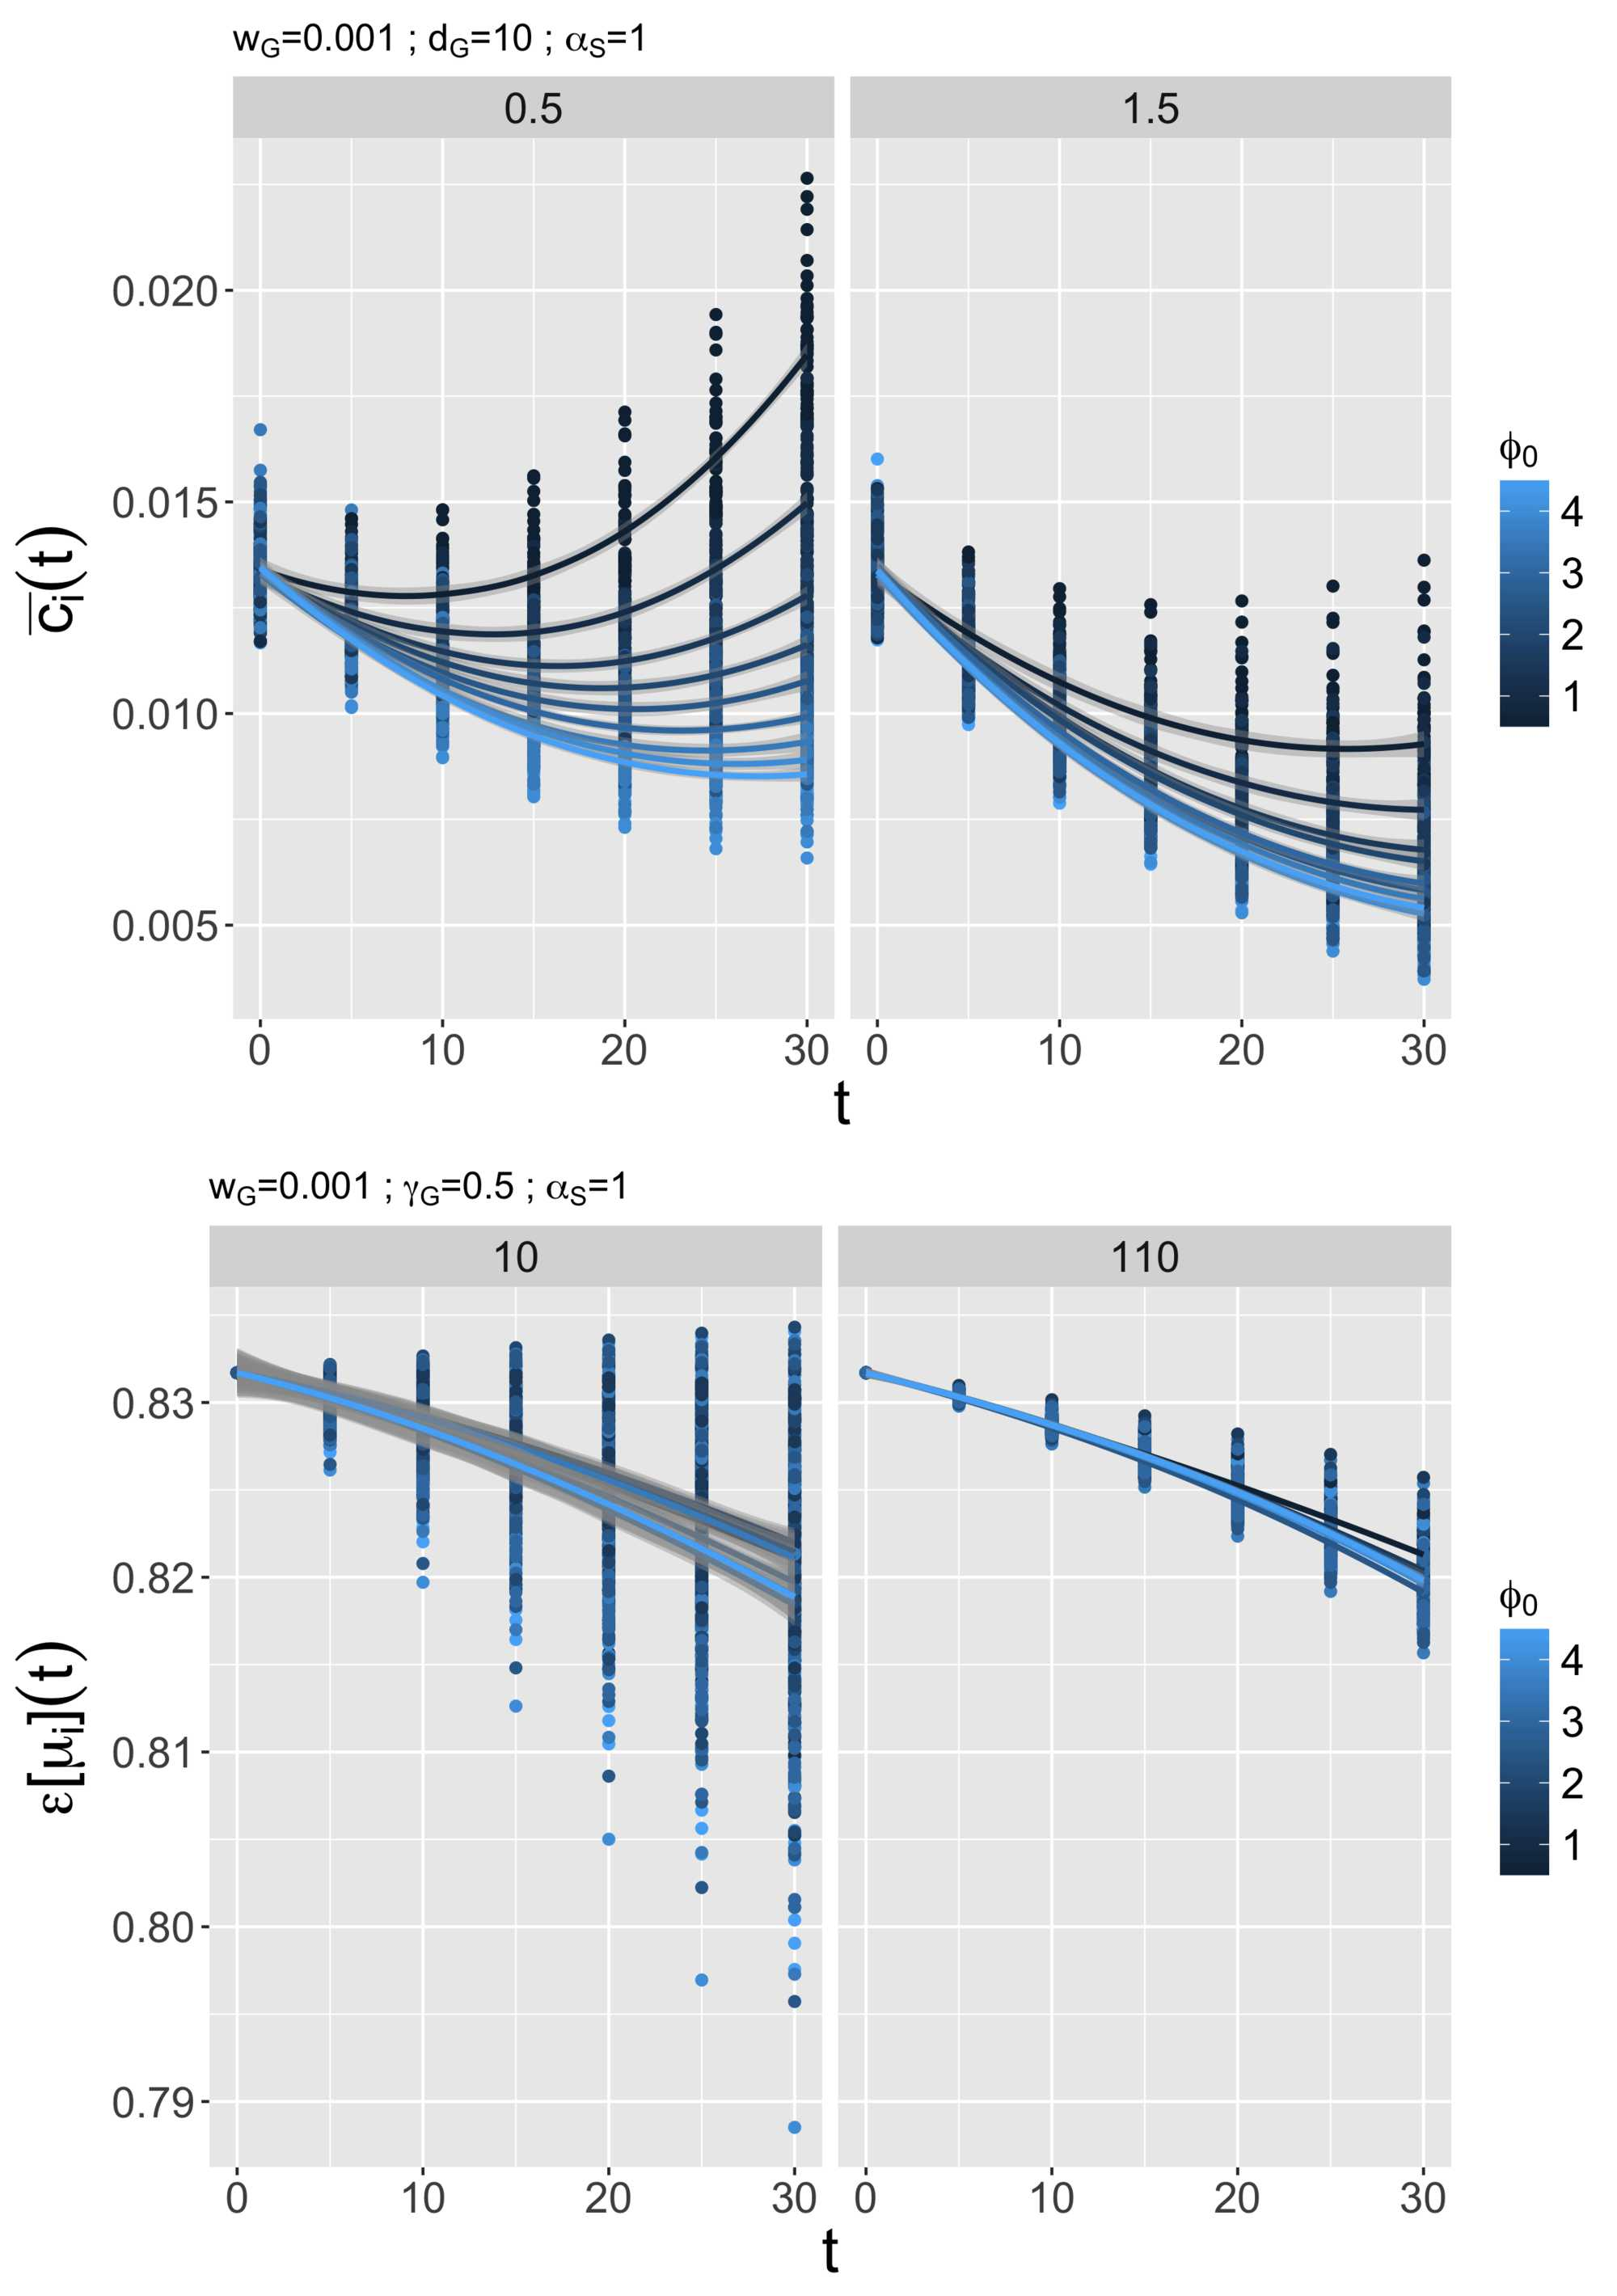
\includegraphics[width=\textwidth]{figures/6-2-2-fig-macrocoevol-behavior-time.jpg}
	\end{column}
	\begin{column}{0.45\linewidth}
		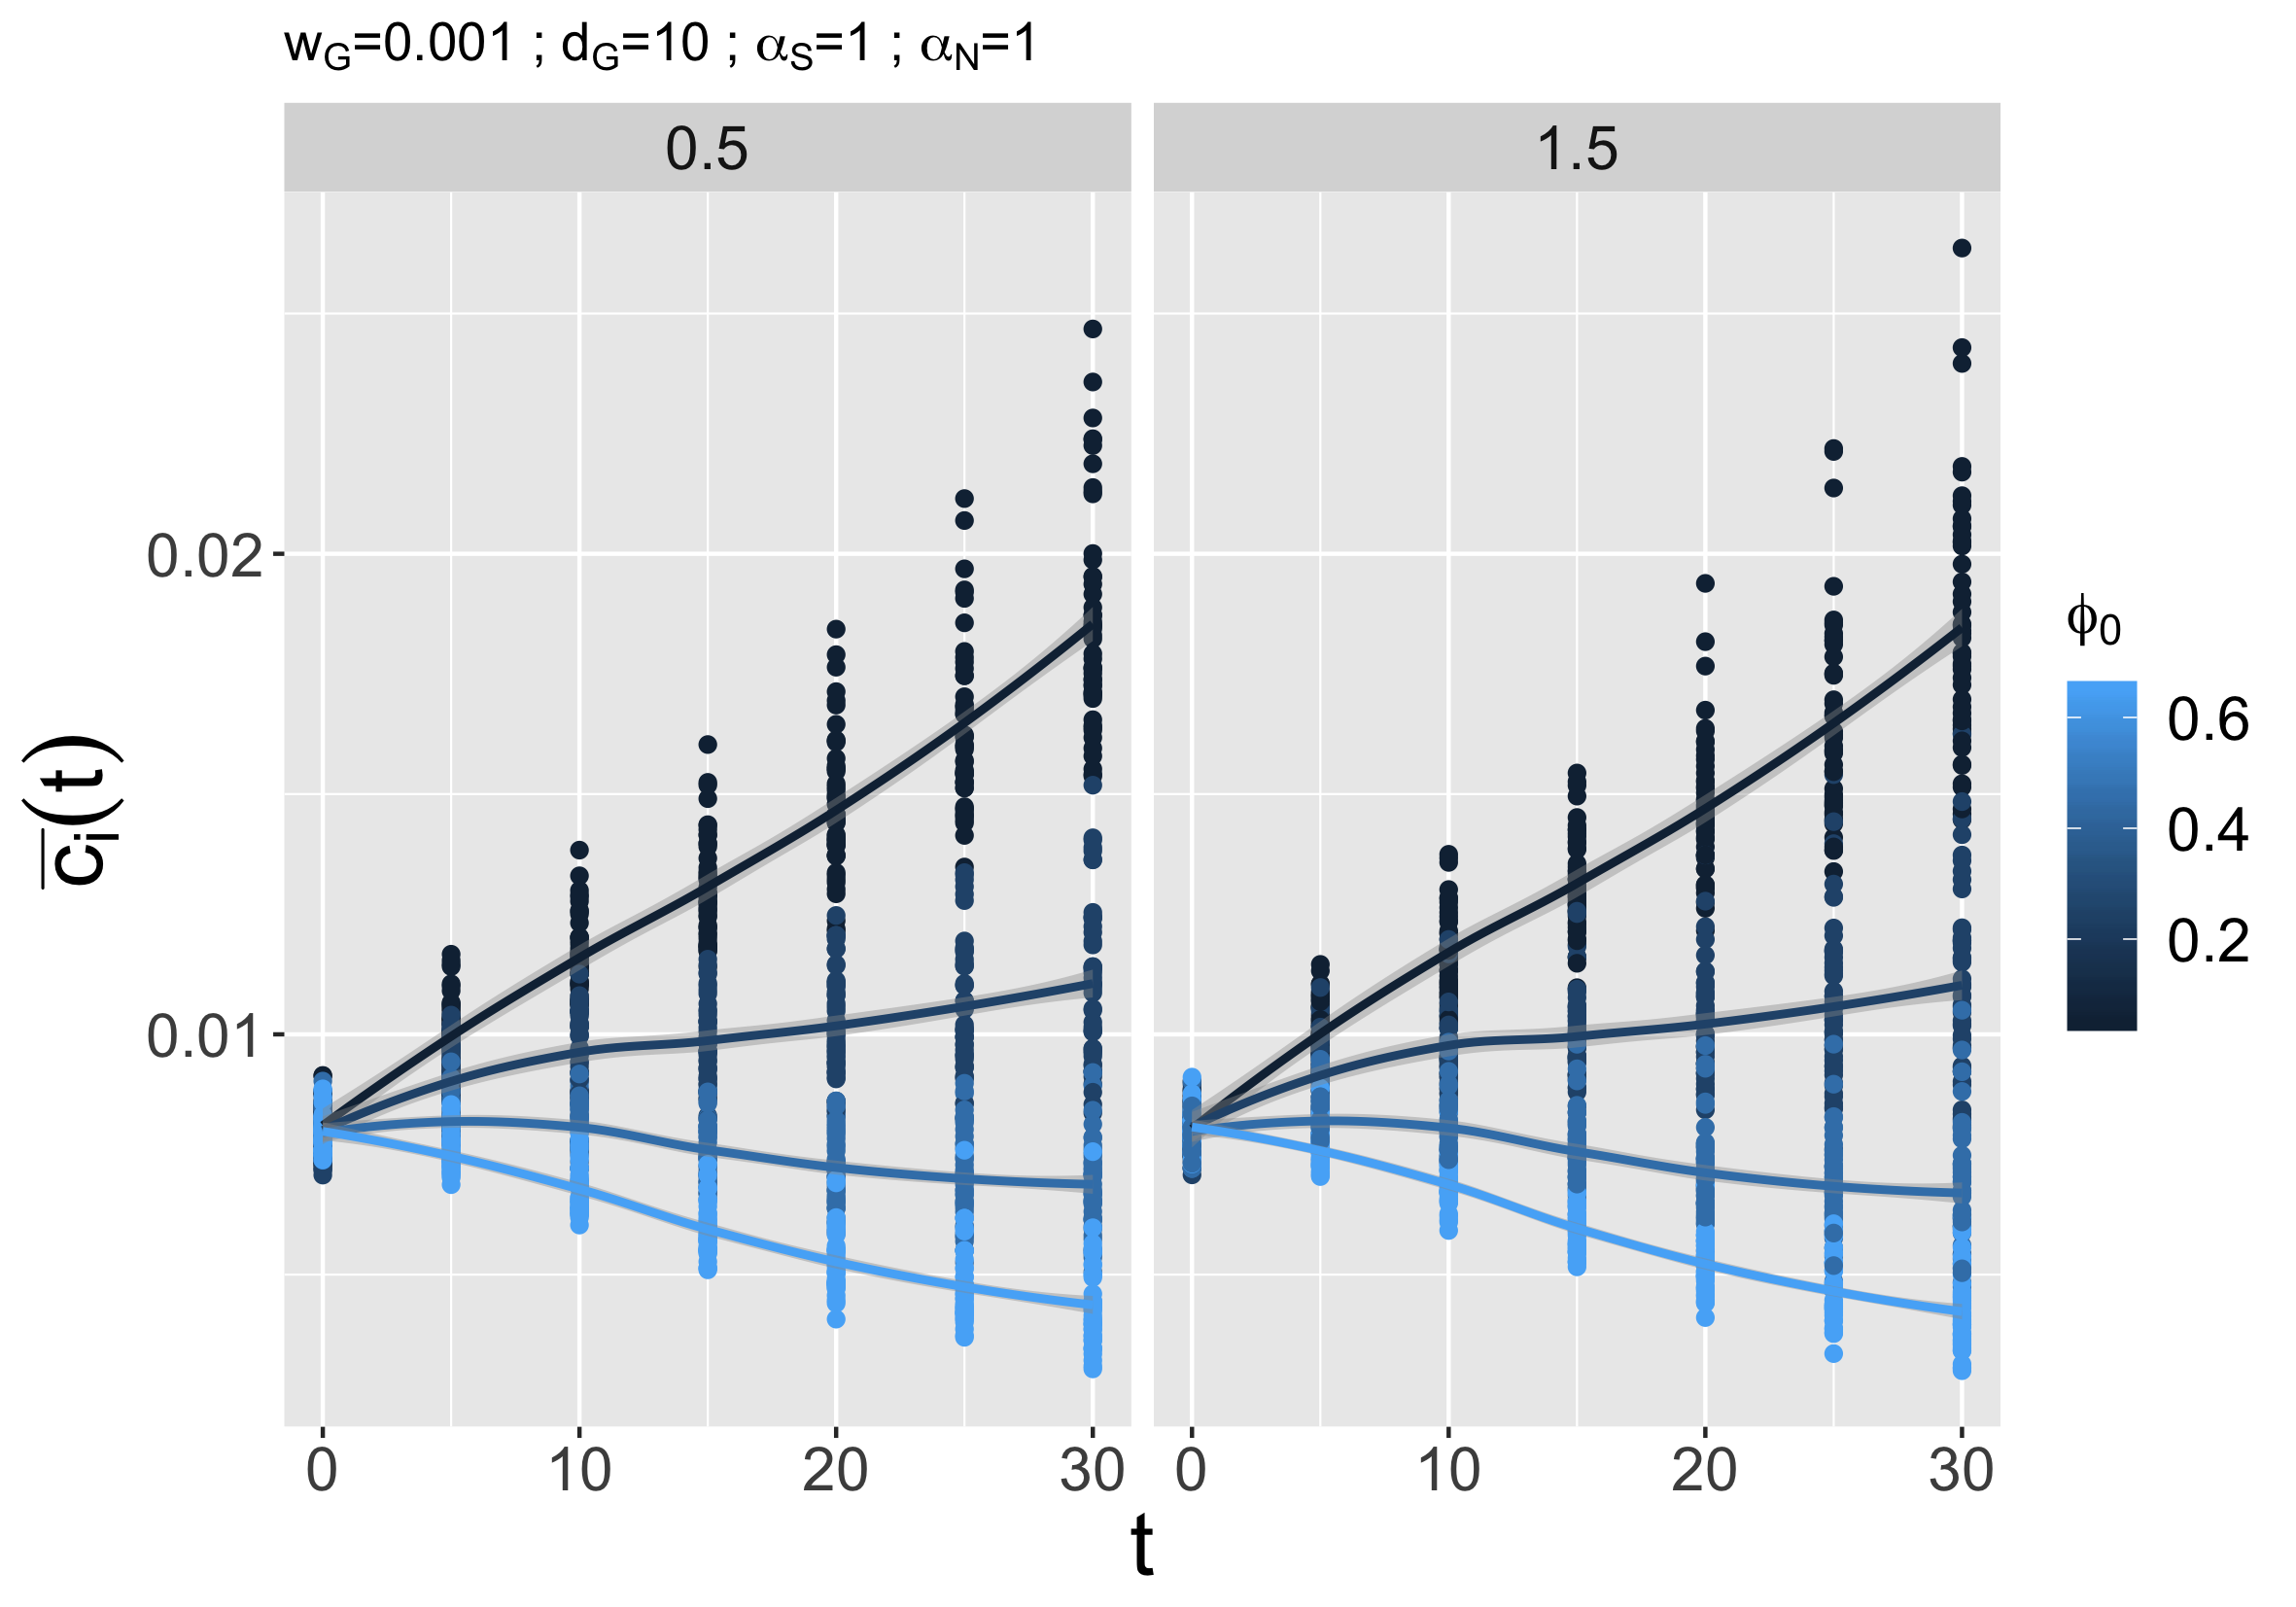
\includegraphics[width=\textwidth]{figures/closenessSummaries_mean_synthRankSize1_gravityWeight0_001_gravityDecay10_nwExponent1.png}\\
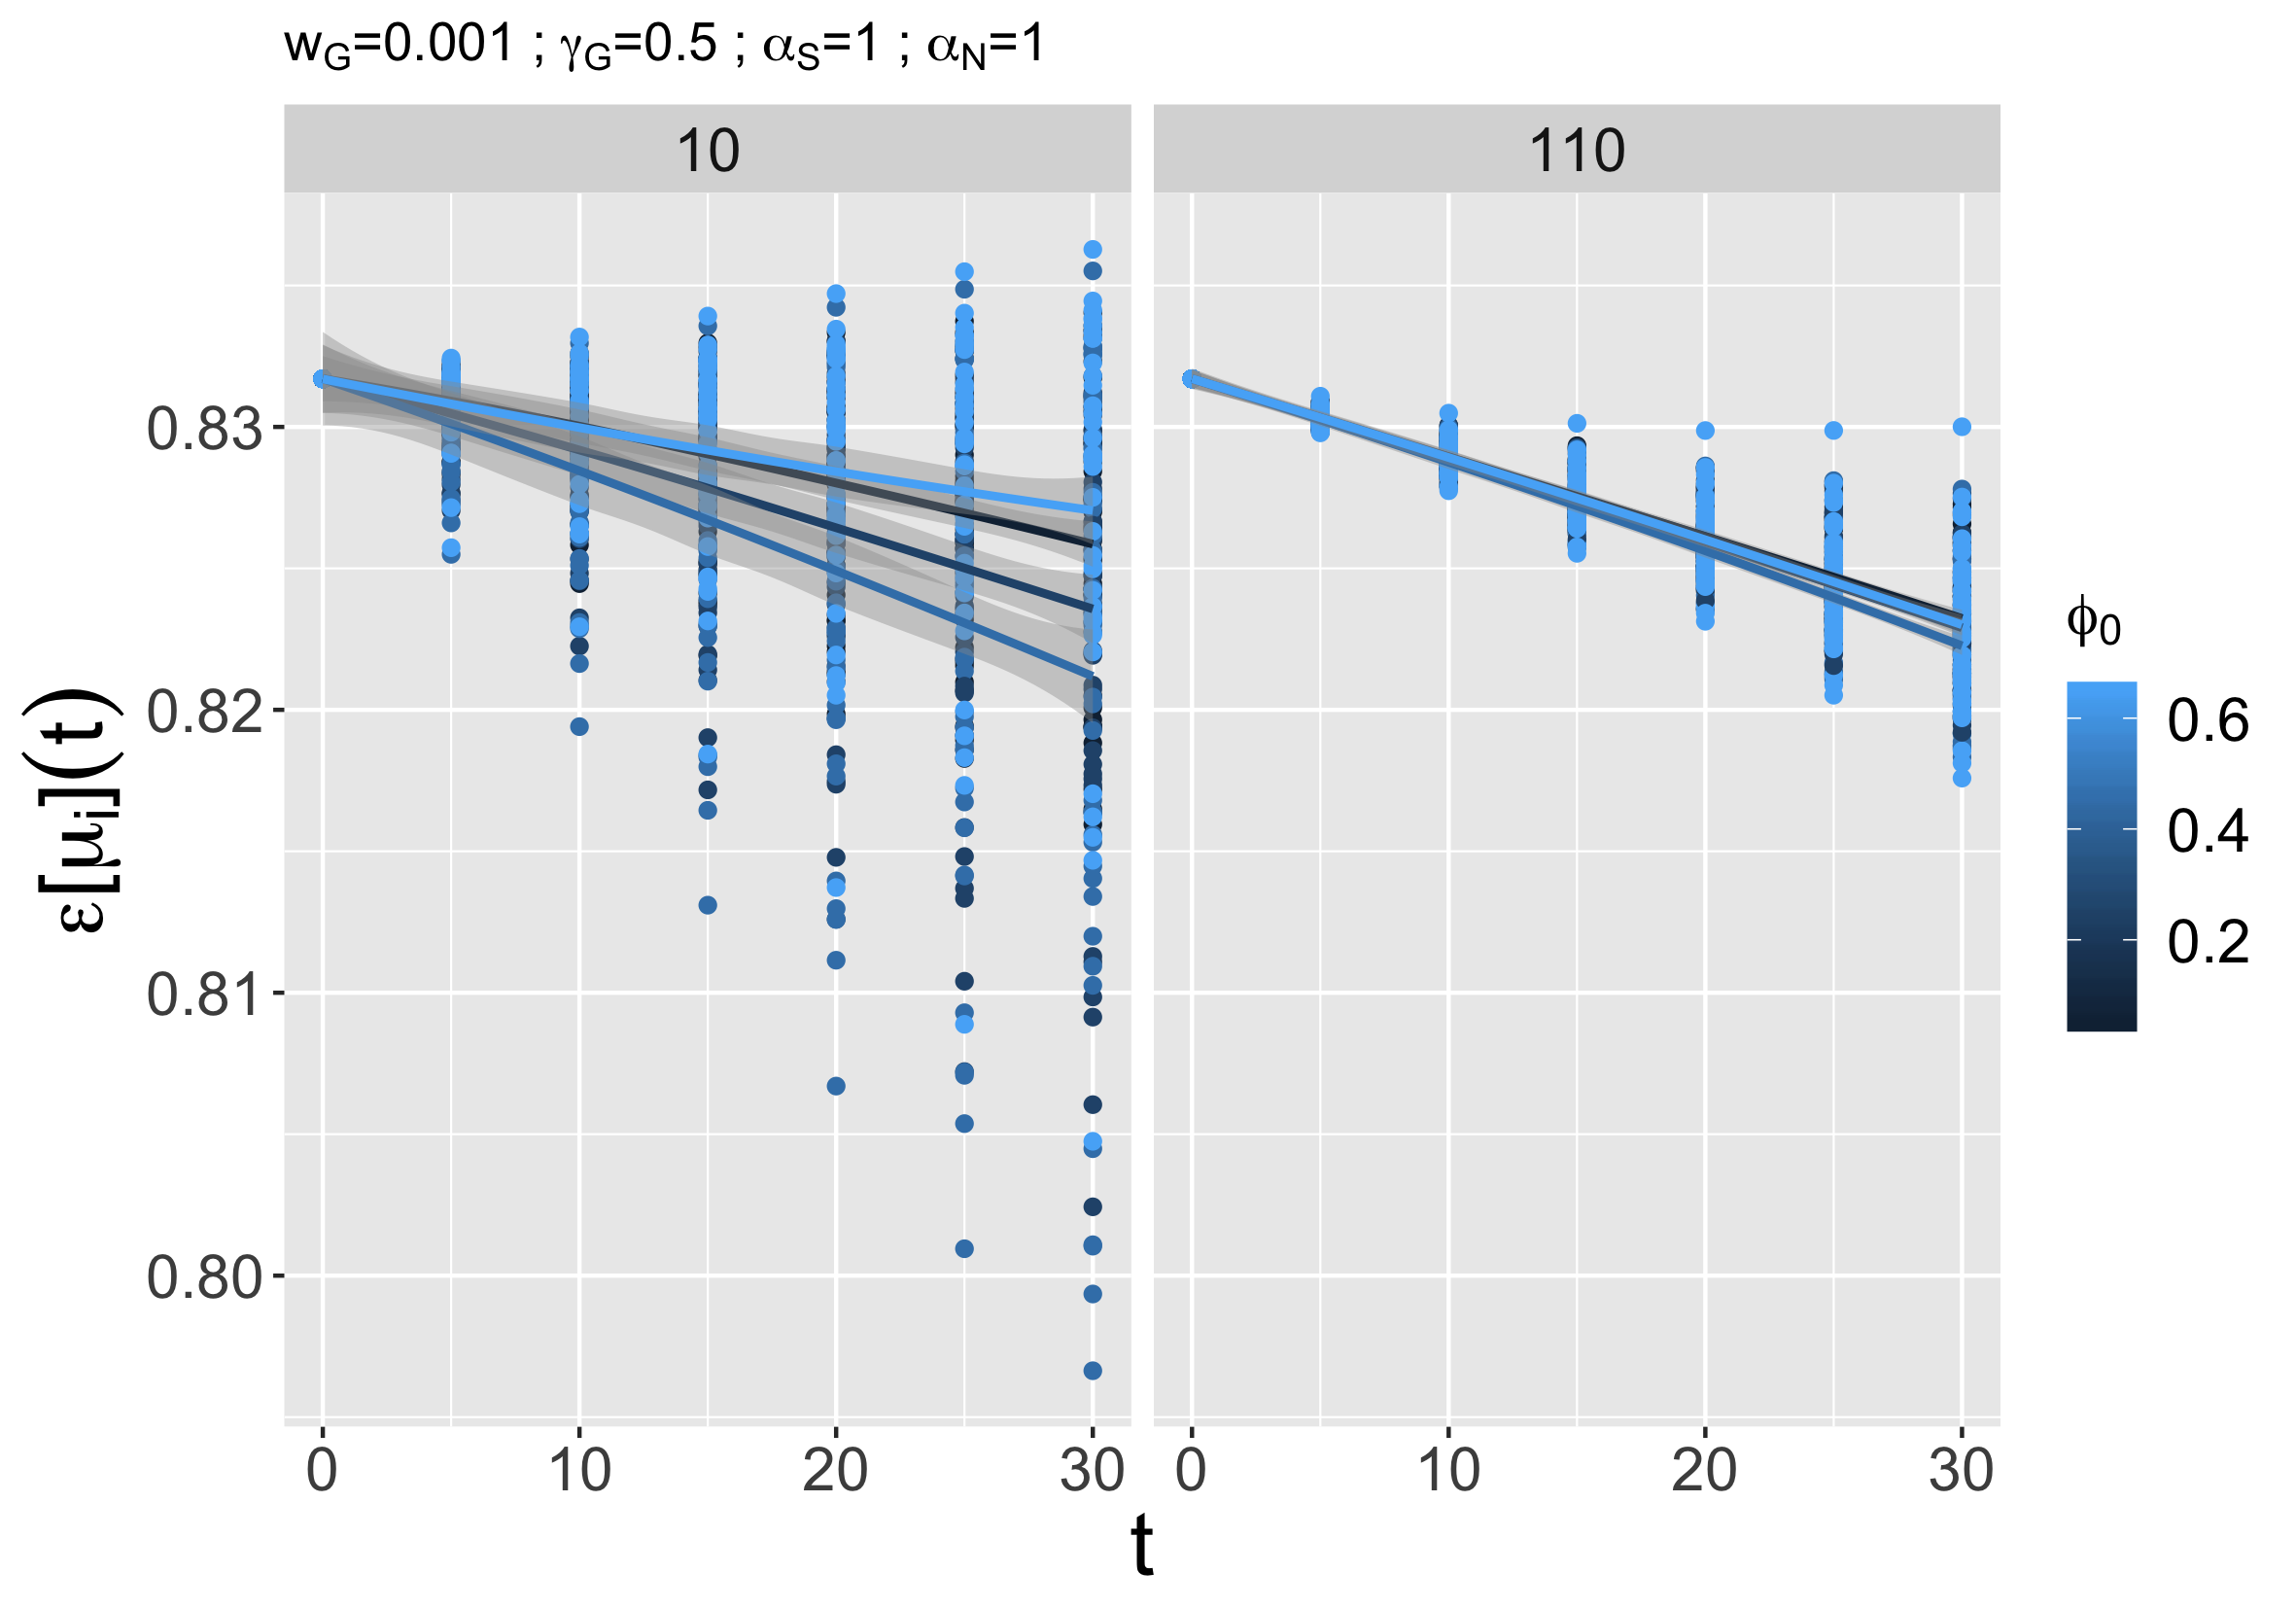
\includegraphics[width=\textwidth]{figures/populationEntropies_synthRankSize1_gravityWeight0_001_gravityGamma0_5_nwExponent1.png}
	\end{column}
\end{columns}

}



\sframe{Model behavior}{

% Systematic explorations of the model on synthetic data using the OpenMole software show that even with the same processes for network growth, qualitative behavior fundamentally differ.
% -> OK ; ex no existence of the complexity maximum

\textit{Strongly different qualitative behavior for aggregated indicators}

\bigskip

\begin{columns}
	\begin{column}{0.5\linewidth}
		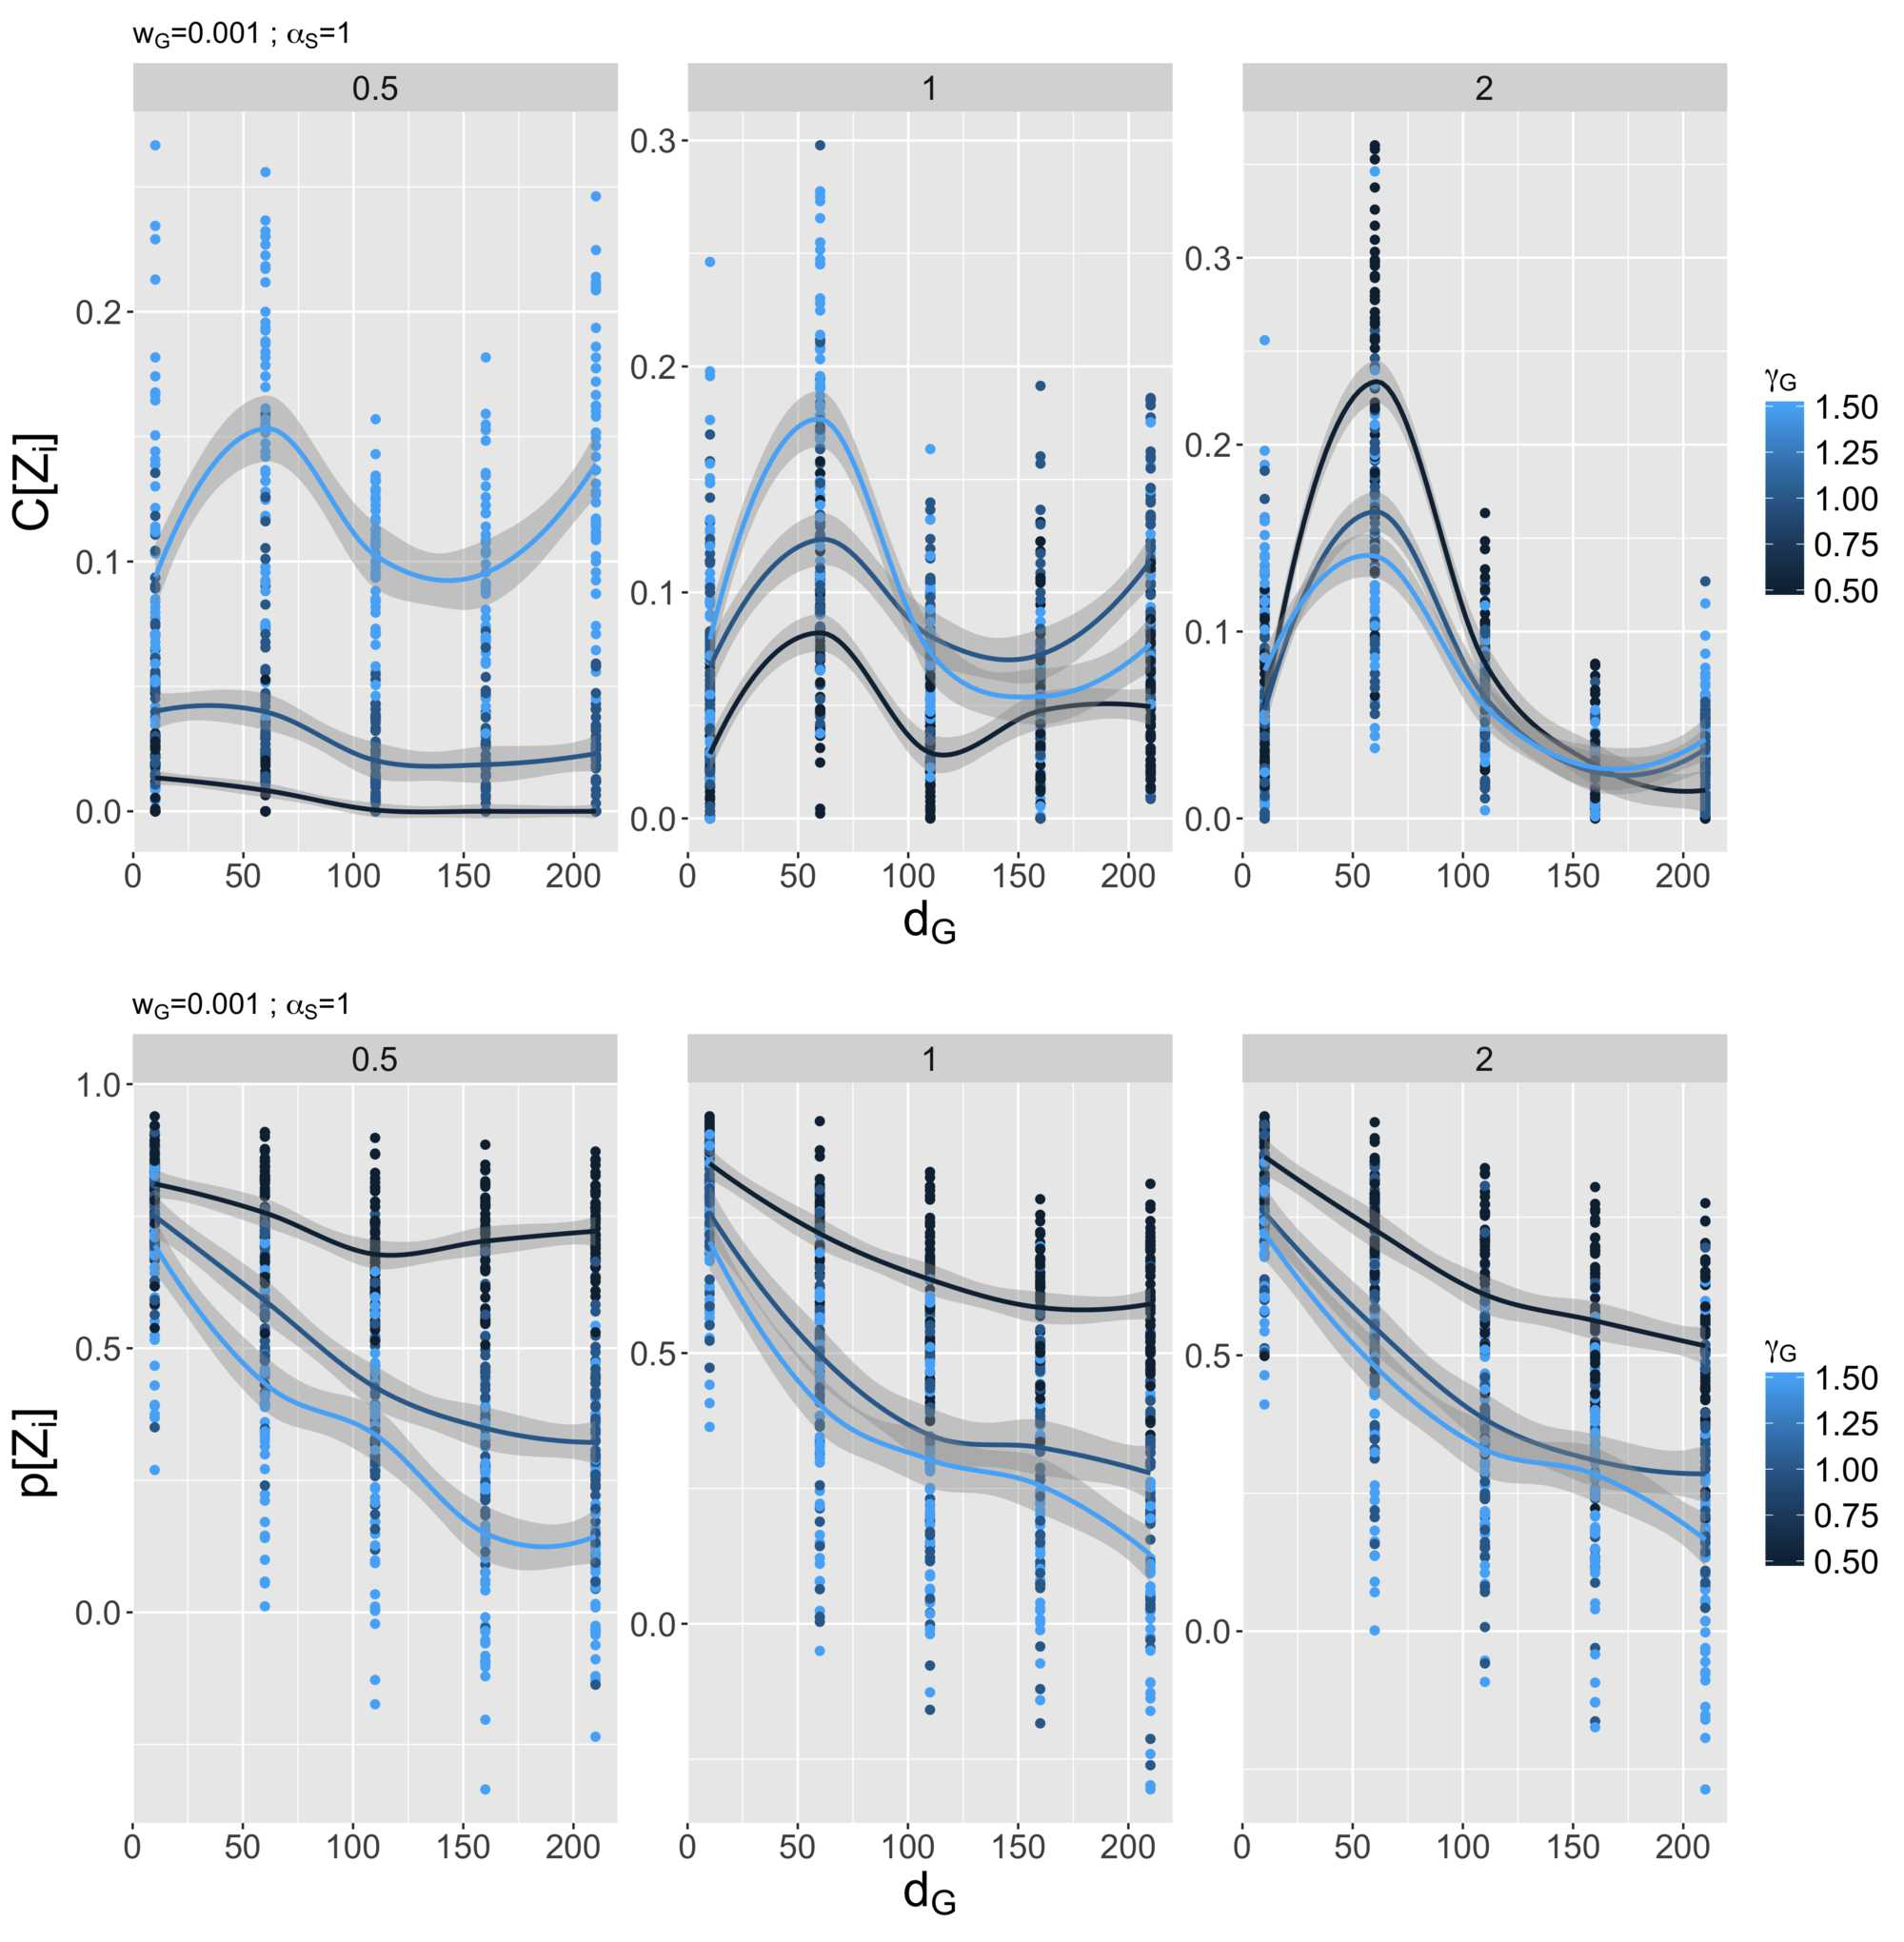
\includegraphics[width=\textwidth]{figures/6-2-2-fig-macrocoevol-behavior-aggreg.jpg}
	\end{column}
	\begin{column}{0.5\linewidth}
		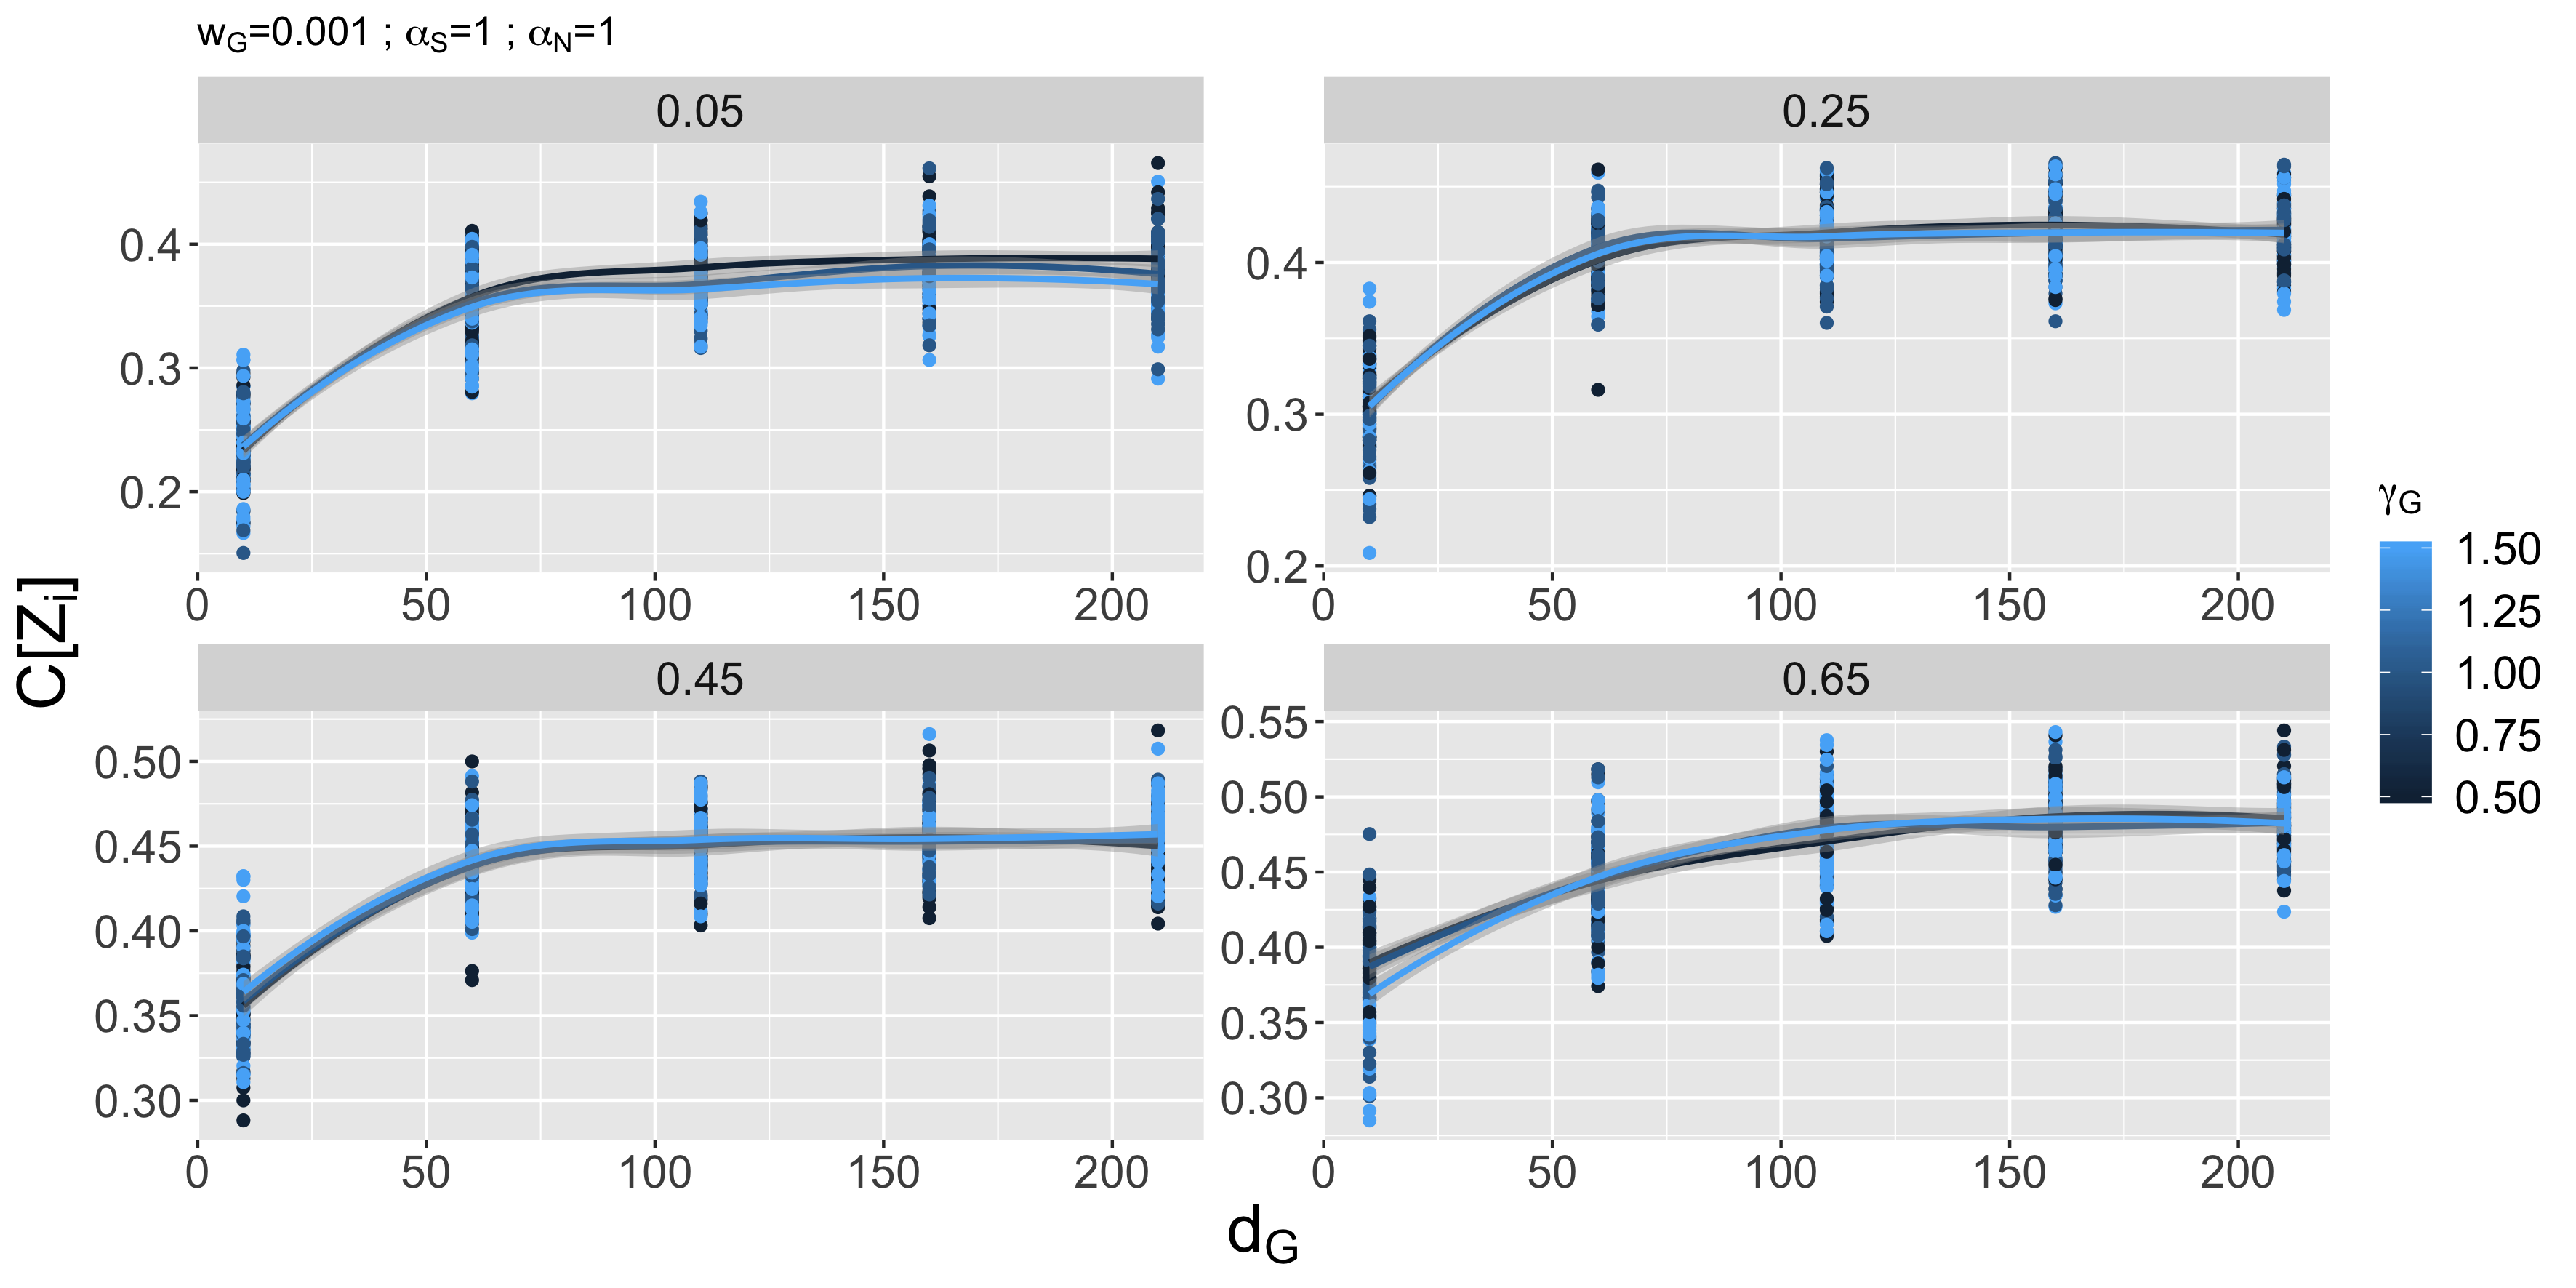
\includegraphics[width=\textwidth]{figures/complexityAccessibility_synthrankSize1_nwGmax0_05_gravityWeight0_001_nwExponent1.png}\\
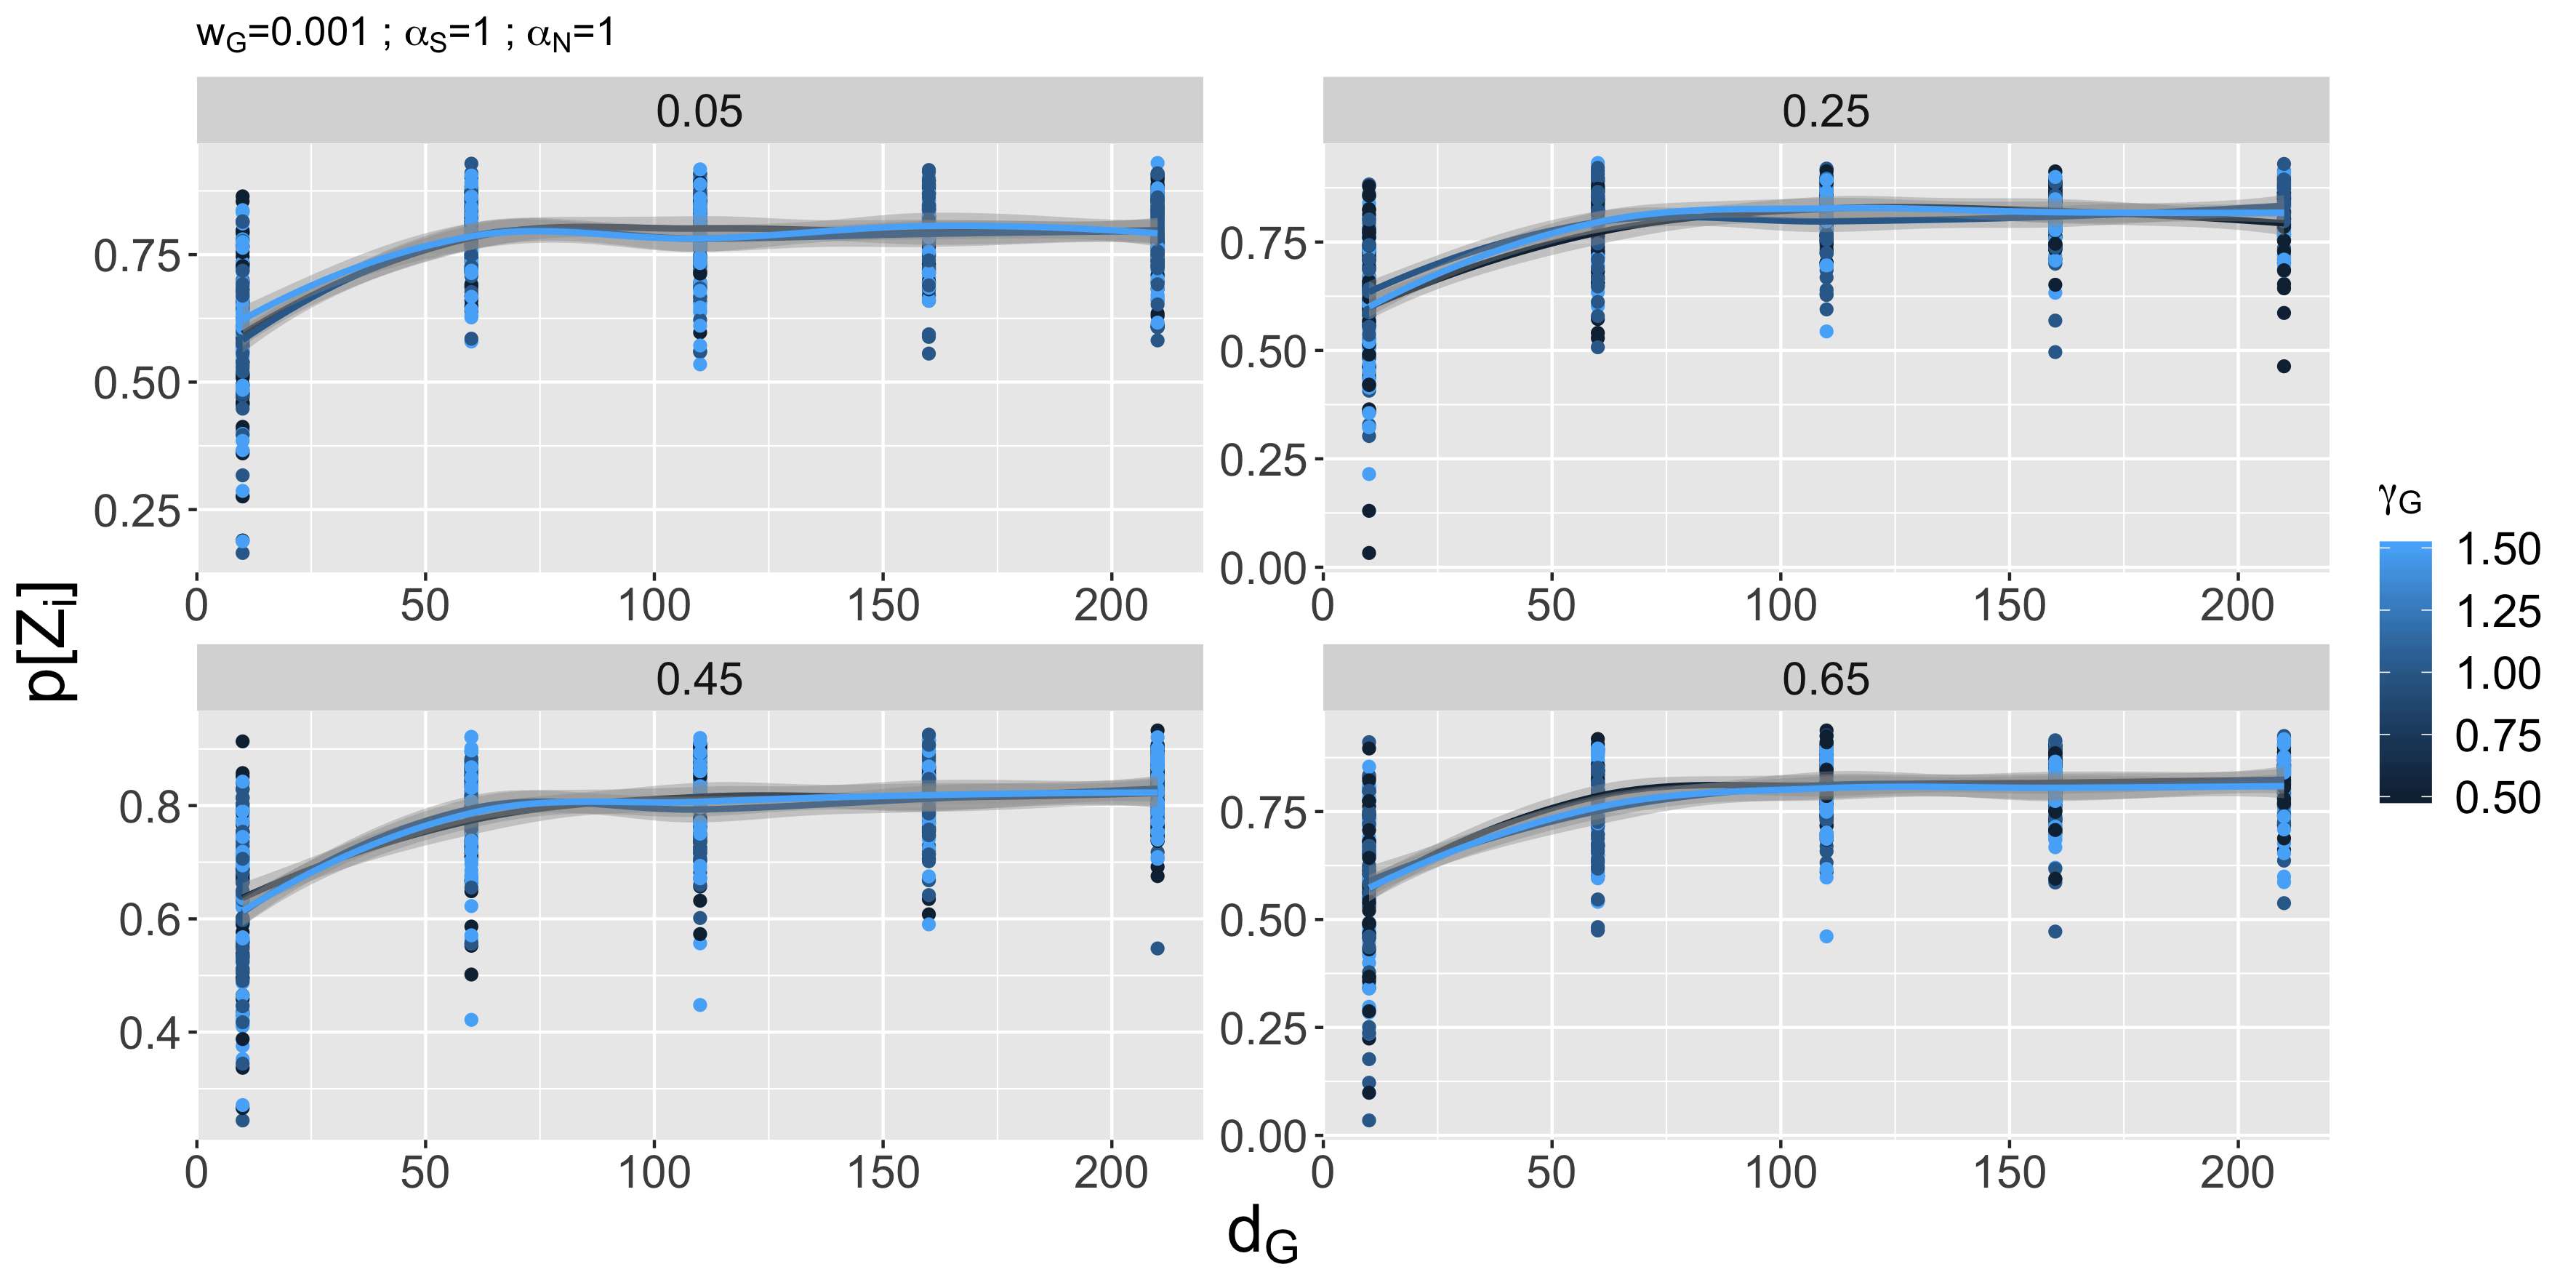
\includegraphics[width=\textwidth]{figures/rankCorrAccessibility_synthrankSize1_nwGmax0_05_gravityWeight0_001_nwExponent1.png}
	\end{column}
\end{columns}


}


\sframe{Interaction regimes}{

%  In particular, co-evolutive dynamics are more difficult to characterize in the hybrid scale models, recalling results obtained by \cite{raimbault2018caracterisation} with the SimpopNet model \cite{schmitt2014modelisation} which has a similar structure.
% -> seems less with grid explo ; may be difficult to say in general (-> PSE needed)

% number of regimes 



%===============
% with 20190201_174314_SYNTHETICPHYSICAL_GRID
% unique(signs$sign)[grep('11',unique(signs$sign))]
%[1] "00/11/11" "00/11/00" "00/01/11"
% -> only three coevolution regimes

% redo with new runs

%===============
% with 20190204_211508_SYNTHETICPHYSICAL_GRID
%unique(signs$sign)[grep('11',unique(signs$sign))]
%[1] "00/01/11" "00/11/01" "00/11/00" "00/11/11"


\justify


\textit{Less co-evolution regimes: similar results than \cite{raimbault2018unveiling} which explored the SimpopNet model} (only 3 against 19 co-evolutive regimes)

\bigskip


\begin{columns}
	\begin{column}{0.5\linewidth}
		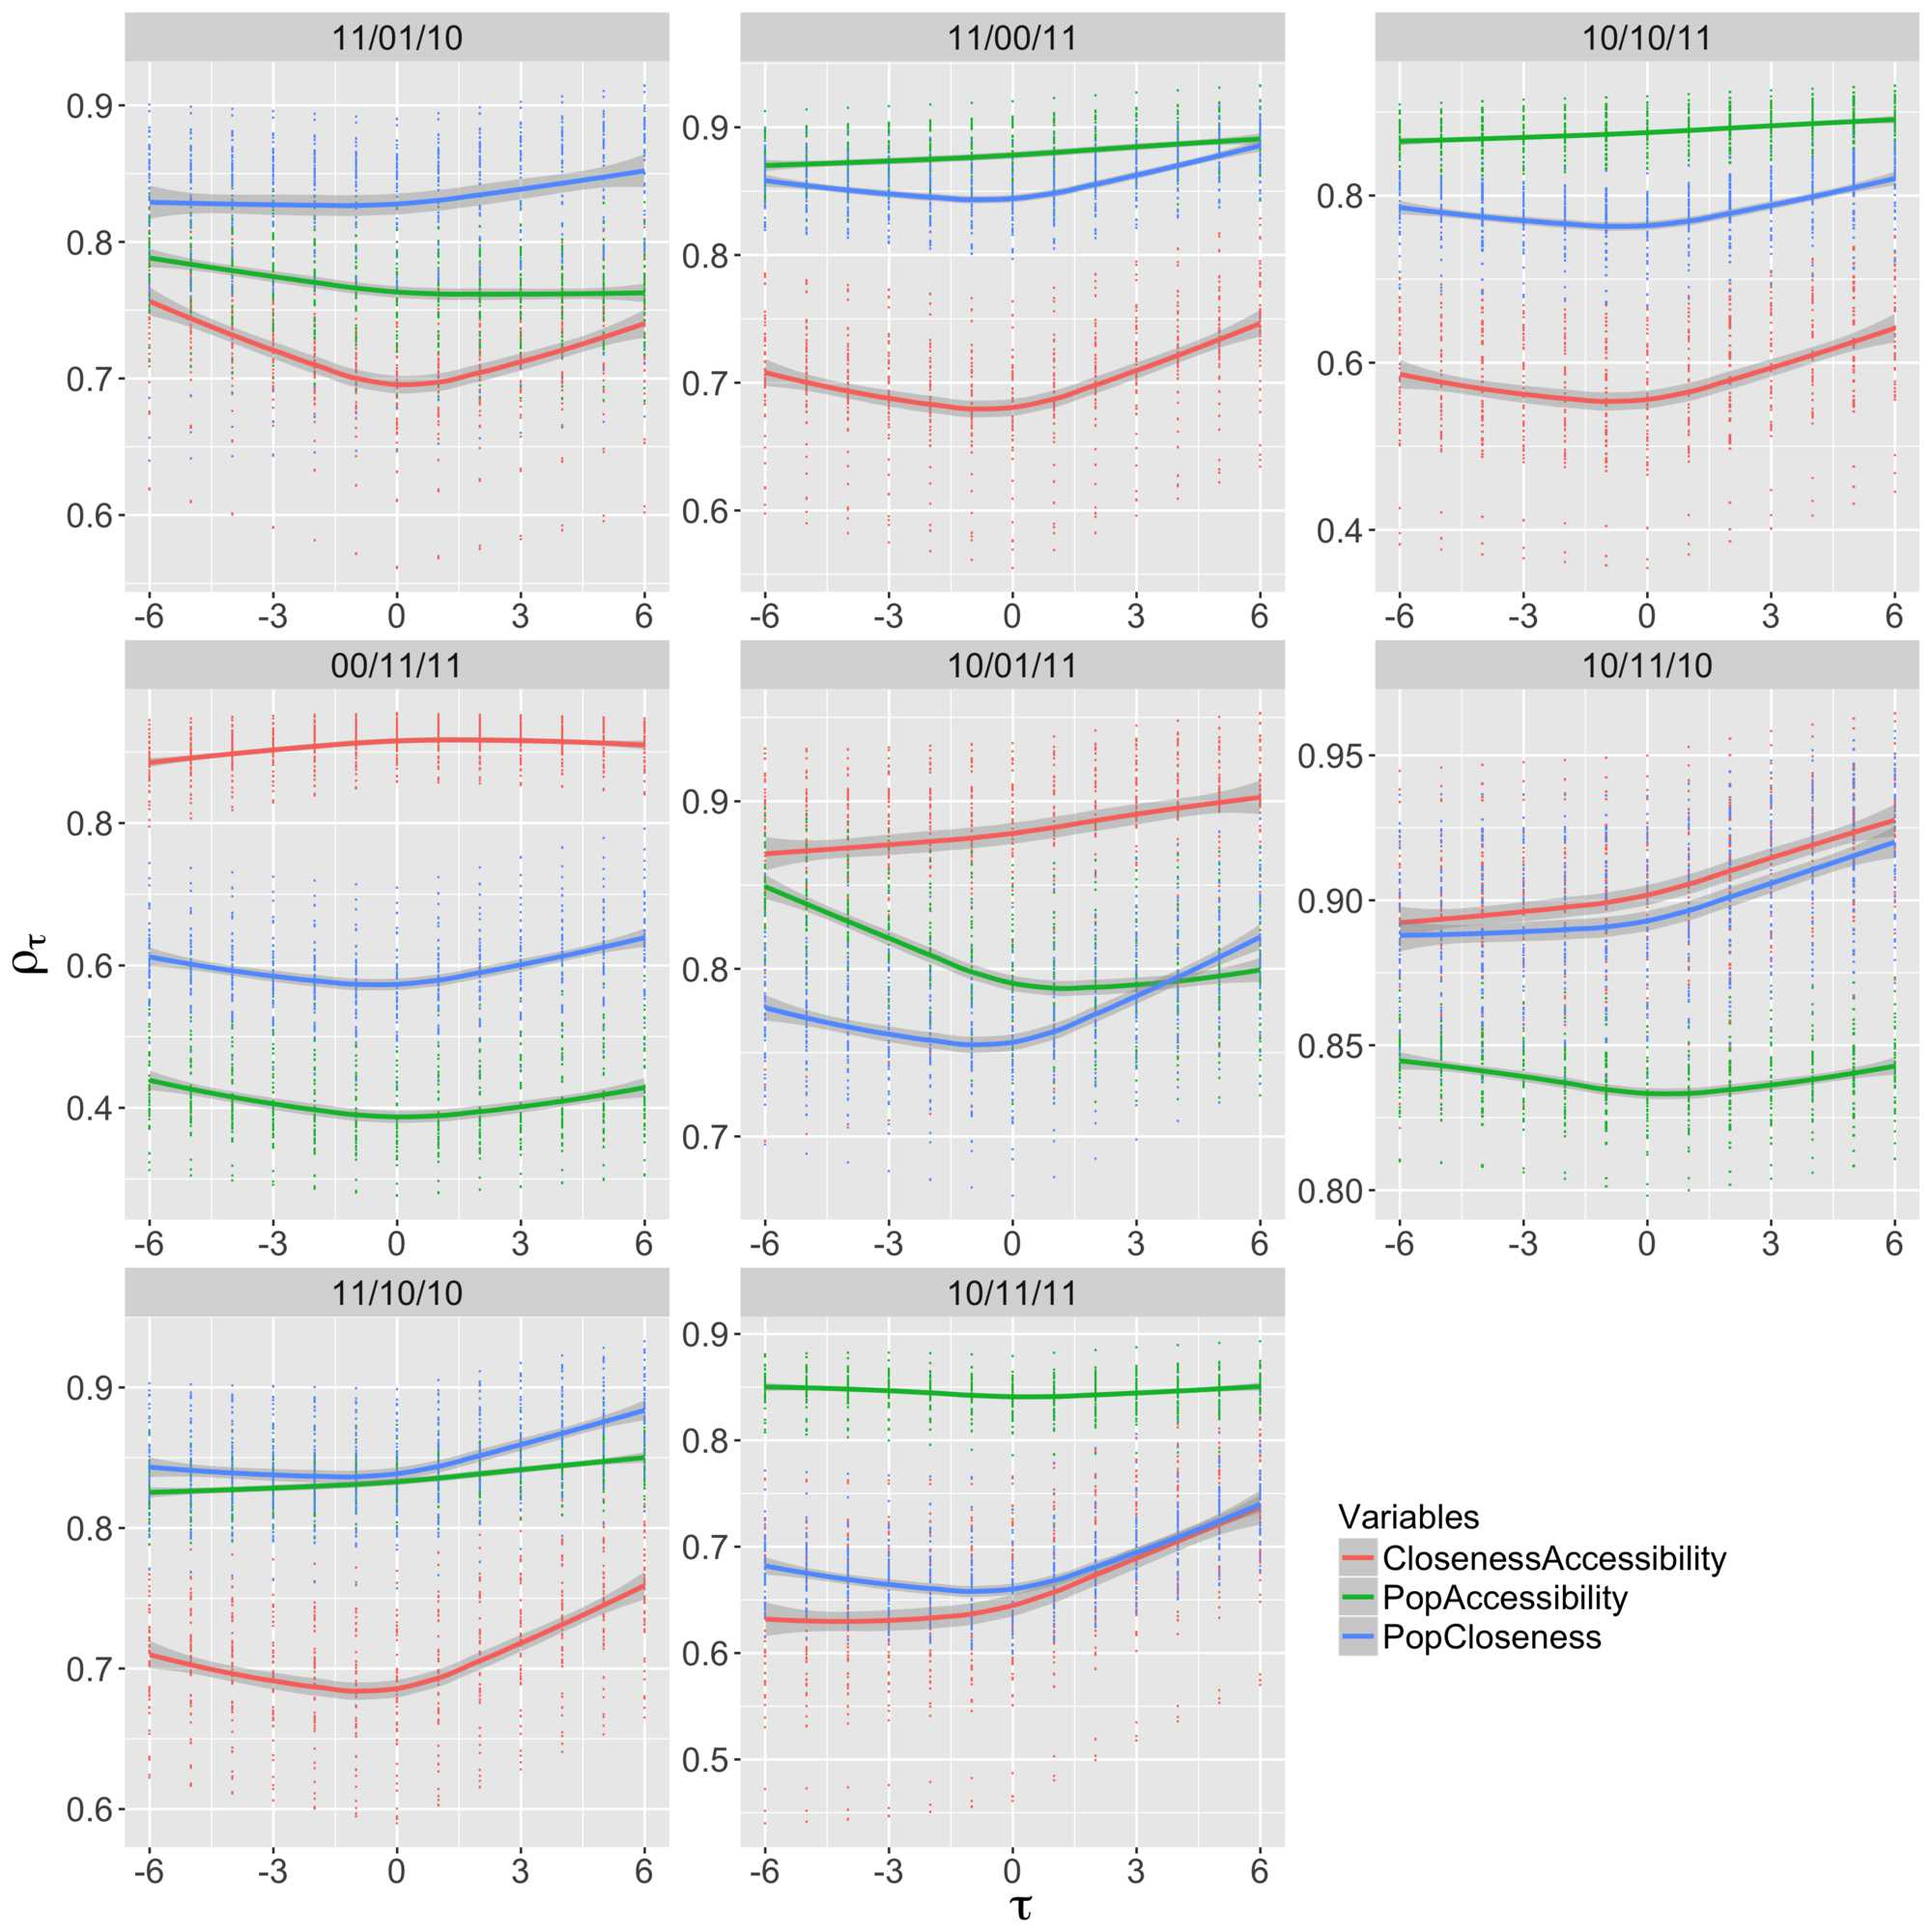
\includegraphics[width=\textwidth]{figures/6-2-2-fig-macrocoevol-correlations.jpg}
	\end{column}
	\begin{column}{0.5\linewidth}
		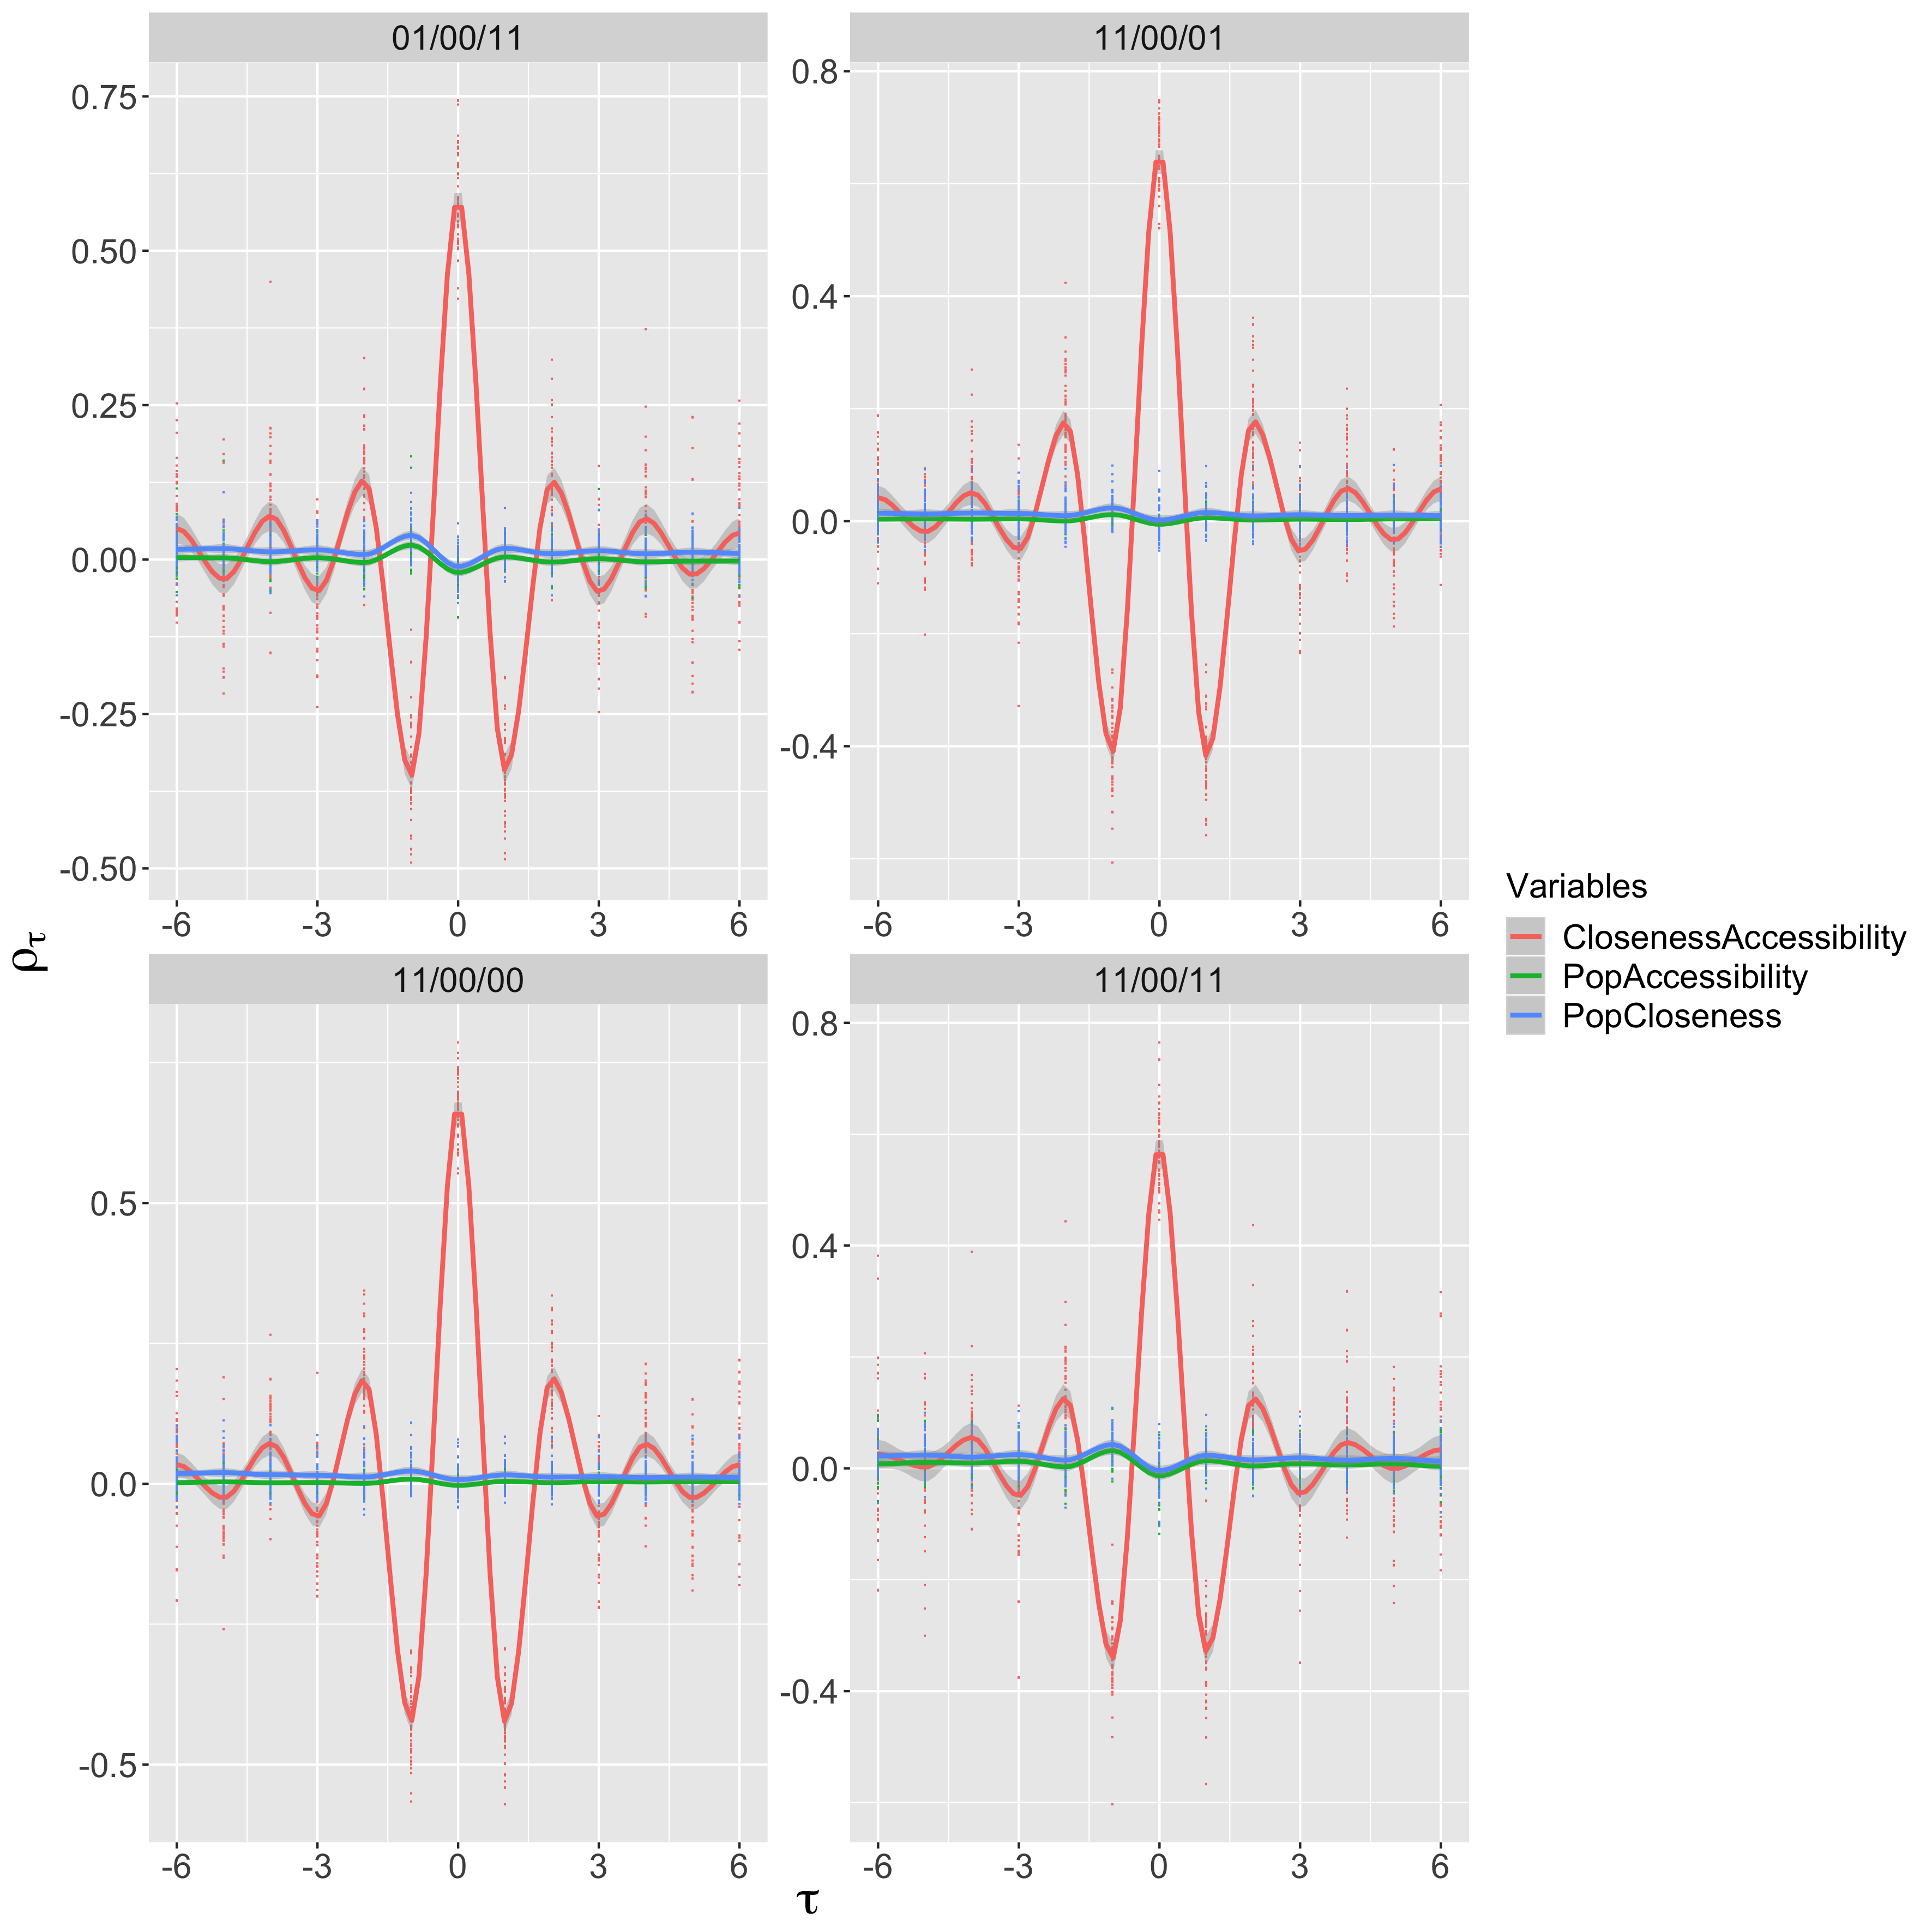
\includegraphics[width=\textwidth]{figures/laggedregimes_absrho_nwGmax0_05.png}
	\end{column}
\end{columns}

% arma(1,1) behavior -> WTF ???

\medskip

\footnotesize \textit{Comparison of regimes with strongest entanglement: auto-correlation bias with virtual network; apparent AR(1) behavior with physical network: sensitivity to indicators definition ?}

% TODO : idee : type de formes des courbes donne une sorte de "meta-regime ?"

}


\sframe{Model calibration}{

% Calibration on the French system of cities with the objective of population and distance matrices accurateness gives mitigated results in comparison to the original model, but however witnesses fit improvement on several temporal calibration windows. These results suggest that the hybrid model would be closer to the actual complexity of these dynamics, as it was shown by \cite{raimbault2018modeling} that co-evolution is indeed difficult to characterize empirically for the French system of cities with railway network data.

% - more constrained physical model ? (rq : no link creation -> the hardest part is still left behind - should couple with an effective network growth model ? )
% - rq : much much better results for abstract flows : few evolutions, do not accurately reflected by flow reinforcement.
% - why so few points on the Pareto front ?

% TODO results calib : latest


\justify

\textit{Much more mediocre results for distance matrices, improvement for population fit on some time windows: converge with the difficulty to characterize co-evolution with the same data \cite{raimbault2018modeling} ?}

\bigskip
\bigskip


\begin{columns}
	\begin{column}{0.53\linewidth}
		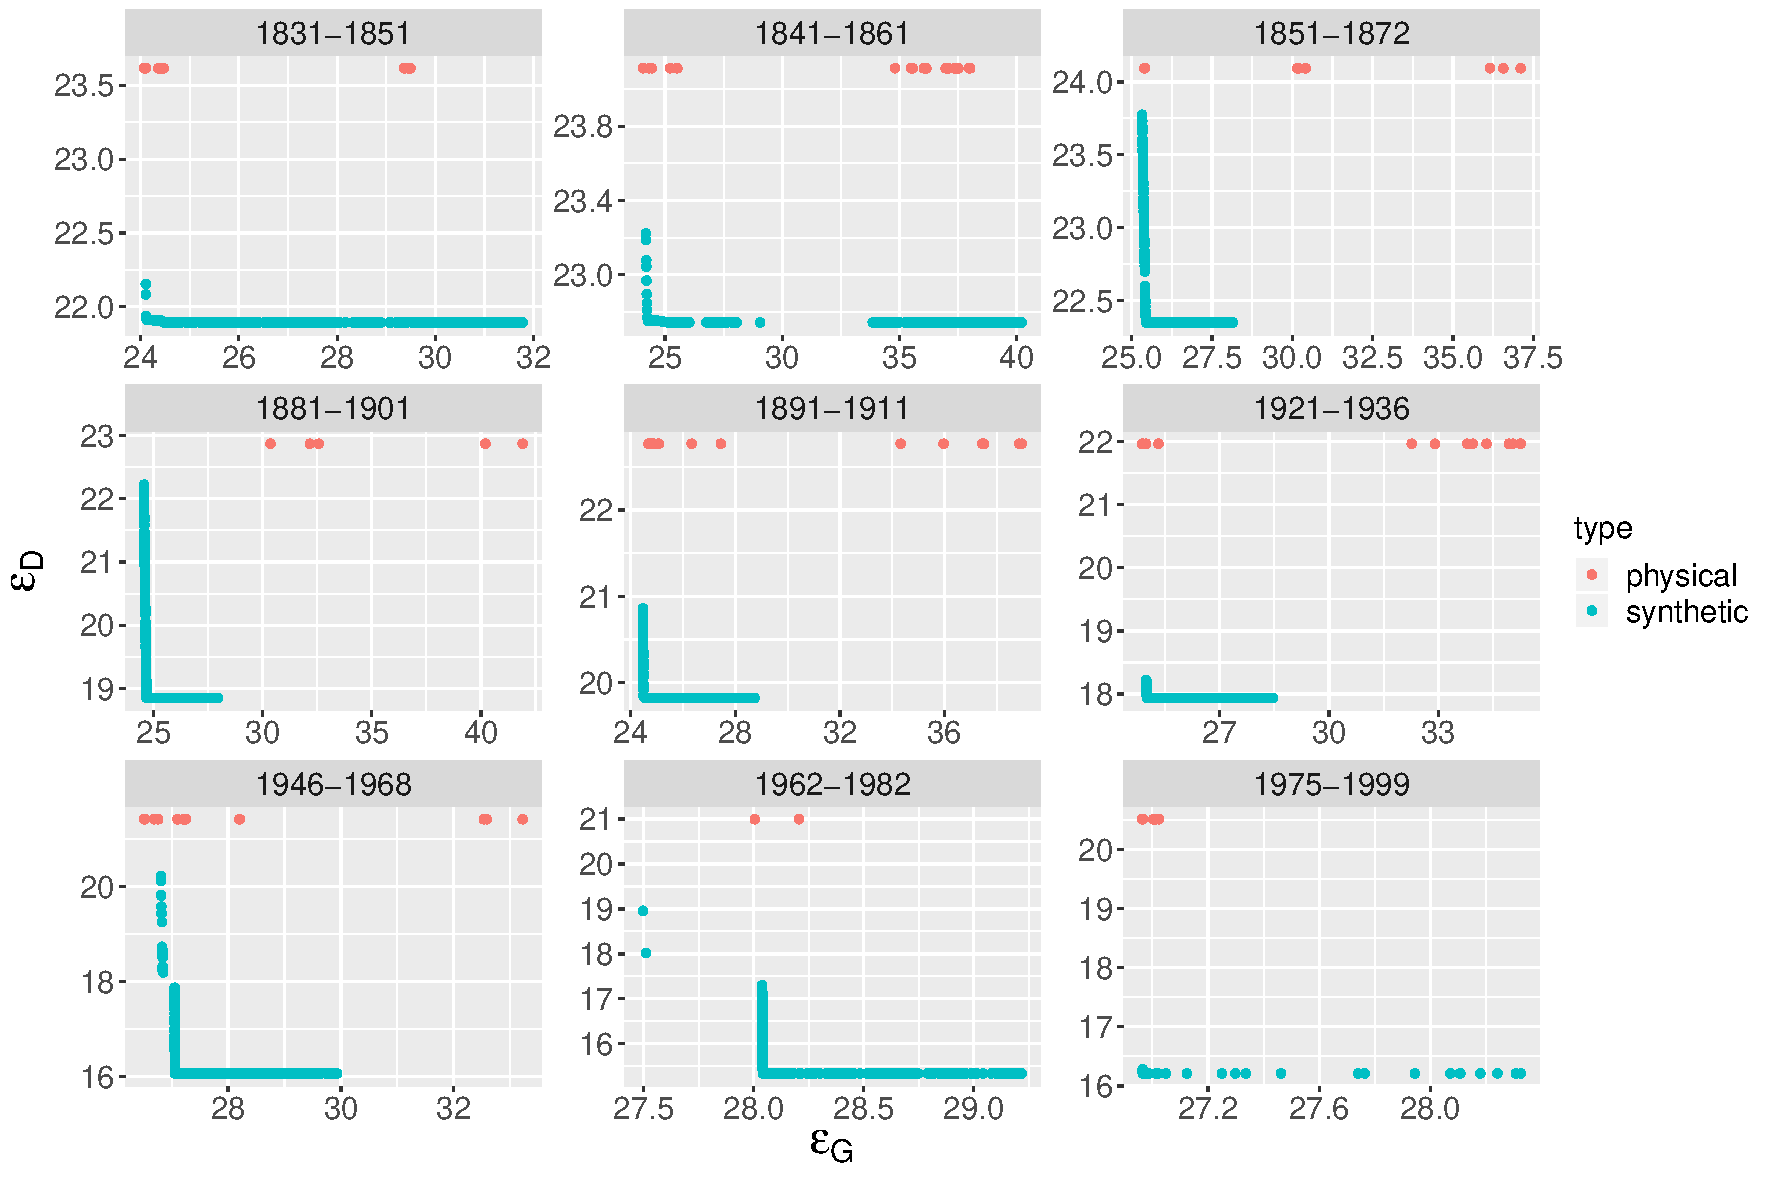
\includegraphics[width=\textwidth]{figures/pareto_comparison_filtFALSE.pdf}
	\end{column}
	\begin{column}{0.53\linewidth}
		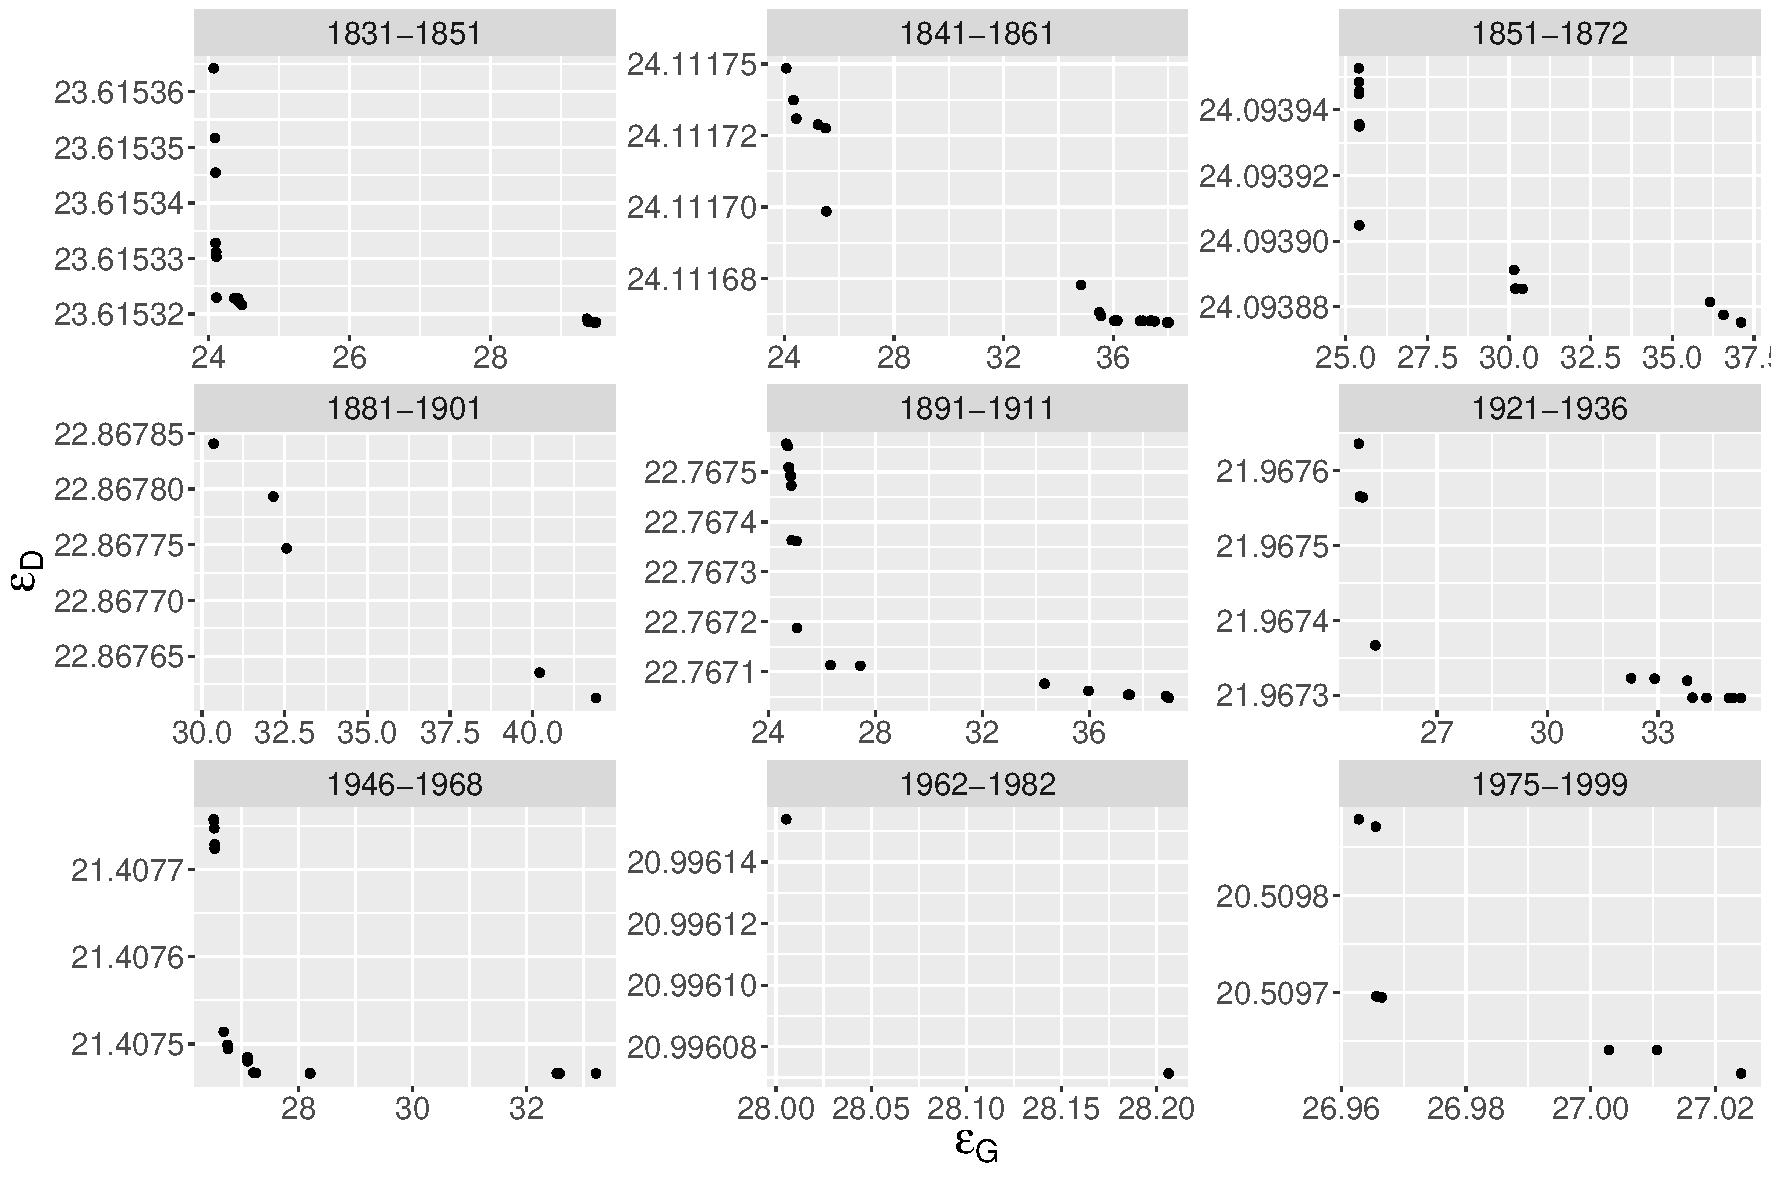
\includegraphics[width=\textwidth]{figures/pareto_filtFALSE.pdf}
	\end{column}
\end{columns}







}


\sframe{Theoretical proposal for a multi-scalar model}{

%   We finally discuss from a theoretical point of view what would be the advantages of a multi-scale coupling of the macroscopic and the mesoscopic model (including for example a more operational character, more accurate conditioning of local dynamics by exogenous parameters determined at the macroscopic scale, a better grasp on spatio-temporal non-stationarity) and present different modeling alternatives that could be followed to achieve this coupling.


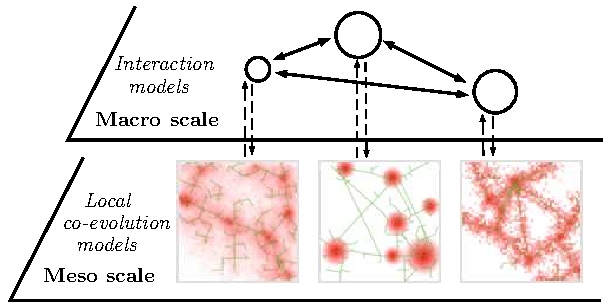
\includegraphics[width=\textwidth]{figures/multiscale.pdf}

\bigskip

\footnotesize

\textit{Several open questions: spatial non-stationarity, nature of inter-scale coupling, level of calibration, operationalization, \ldots}

}




\sframe{Discussion}{

\justify

\textbf{Implications}

\medskip

$\rightarrow$ Such hybrid models closer or further to the actual complexity of co-evolution ?

\medskip

$\rightarrow$ Implications for planning still to be determined (two different policy type and level)


\bigskip

\textbf{Developments}

\medskip

% cf simpopnet chapter
$\rightarrow$ Fair comparison of number of interaction regimes using PSE algorithm \cite{10.1371/journal.pone.0138212}; fair comparison of calibrations taking into account number of parameters \cite{piou2009proposing}

\medskip

$\rightarrow$ Multi-modeling for network growth in the hybrid model, including topological evolution \cite{raimbault2018multi}

\medskip

$\rightarrow$ Towards the inclusion of governance processes in co-evolution models \cite{lenechet:halshs-01272236}



}




\section{Conclusion}


\sframe{Conclusion}{

\justify

\small

$\rightarrow$ Towards multi-scalar models and multi-models, calibrated on several systems of cities \cite{raimbault2018systematic}: foundations of integrative models for territorial systems


\medskip

$\rightarrow$ Towards an integration of complexities \cite{raimbault2018relating} \cite{2019arXiv190109869R}: foundations of integrative theories of territorial systems 
%Réflexivité (entre autre complexité appliquée à la complexité) nécessaire pour une connaissance complexe \cite{morin1991methode} ; vers un perspectivisme appliqué ? \cite{banos2018spatialised}
%Vers une intégration plus systématique (épistémologiquement et théoriquement) des différentes complexités pour l'étude des systèmes territoriaux ? \\\cite{raimbault2018relating}

\bigskip

\footnotesize

\textbf{Some references}

%Raimbault, J. (2018). Calibration of a density-based model of urban morphogenesis. PloS one, 13(9):e0203516

%\smallskip

Raimbault, J. (2018). Indirect evidence of network effects in a system of cities. Environment and Planning B: Urban Analytics and City Science, 2399808318774335.

\smallskip

Raimbault, J. (2019). An Urban Morphogenesis Model Capturing Interactions Between Networks and Territories. In L. D'Acci (ed.), The Mathematics of Urban Morphology. Springer Nature Switzerland AG.

\smallskip

Raimbault, J. (2019). Modeling the co-evolution of cities and networks. Forthcoming in Handbook of Cities and Networks, Rozenblat C., Niel Z. (eds.), Edward Elgar Publishing.

%\smallskip

%Raimbault, J., Banos, A., \& Doursat, R. (2014, June). A Hybrid Network/Grid Model of Urban Morphogenesis and Optimization. In 4th International Conference on Complex Systems and Applications (pp. 51-60).

\bigskip
\bigskip


% + dataverse
\footnotesize{ - Code, data and results at\\\texttt{https://github.com/JusteRaimbault/CoevolutionNwTerritories}\\
- Acknowledgements to the \textit{European Grid Infrastructure} and its \textit{National Grid Initiatives} (\textit{France-Grilles} in particular) for the technical support and the infrastructure.

}

}




\sframe{Reserve slides}{
	
	\centering
	
	\Large

\textbf{Reserve Slides}
	
}



\sframe{Macroscopic Interaction Model Rationale}{

\justify

%% bit of theory

\textbf{Rationale :} extend an interaction model for system of cities by including physical network as an additional carrier of spatial interactions

\bigskip

$\rightarrow$ Work under Gibrat independence assumptions, i.e. $\Covb{P_i(t)}{P_j(t)}=0$. If $\vec{P}(t+1)=\mathbf{R}\cdot \vec{P}(t)$ where $\mathbf{R}$ is also independent, then $\Eb{\vec{P}(t+1)}=\Eb{\mathbf{R}}\cdot\Eb{\vec{P}}(t)$. Consider expectancies only (higher moments computable similarly)

\medskip

$\rightarrow$ With $\vec{\mu}(t)=\Eb{\vec{P}(t)}$, we generalize this approach by taking $\vec{\mu}(t+1)=f(\vec{\mu}(t))$


}


\sframe{Macroscopic Model Description}{

Let $\vec{\mu}(t)=\Eb{\vec{P}(t)}$ cities population and $(d_{ij})$ distance matrix


\medskip

Model specified by

\[
f(\vec{\mu}) = r_0\cdot \mathbf{Id}\cdot \vec{\mu} + \mathbf{G}\cdot \mathbf{1} + \mathbf{N}
\]

 with 
\begin{itemize}
\item $G_{ij} = w_G\cdot \frac{V_{ij}}{<V_{ij}>}$ and $V_{ij} = \left(\frac{\mu_i\mu_j}{\sum{\mu_k}^2}\right)^{\gamma_G} \exp{(-d_{ij}/d_G)}$
\item $N_{i} = w_N \cdot \sum_{kl} \left(\frac{\mu_k\mu_l}{\sum\mu}\right)^{\gamma_N}\exp{(-d_{kl,i})/d_N}$ where $d_{kl,i}$ is distance to shortest path between $k,l$ computed with slope impedance ($Z=\left(1+\alpha/\alpha_0\right)^{n_0}$ with $\alpha_0\simeq 3$)
\end{itemize}

}

\sframe{Model Formalization : Network Growth}{

Given the flow $\phi$ in a link, its effective distance is updated following

\begin{enumerate}
\item For the thresholded case
\[
d(t+1) = d(t)\cdot \left( 1 + g_{max} \cdot \left[\frac{1 - \left(\frac{\phi}{\phi_0}\right)^{\gamma_s}}{1 + \left(\frac{\phi}{\phi_0}\right)^{\gamma_s}}\right]\right)
\]
\item For the full growth case
\[
d(t+1) = d(t)\cdot \left(1 + g_{max} \cdot \left[\frac{\phi}{\max \phi}\right]^{\gamma_s}\right)
\]
\end{enumerate}

where $\gamma_s$ is a hierarchy parameter, $\phi_0$ a threshold parameter and $g_{max}$ the maximal growth rate easily adjustable to realistic values by computing $(1+g_{max})^{t_f}$
%
%
%


}


\sframe{Model Description : Indicators}{
  \begin{itemize}
  \item Hierarchy, Entropy, Summary statistics in time
  \item Initial-final rank correlation (changes in the hierarchy) for variable $X$ : $\rho\left[X_i(t=0),X_i(t=t_f)\right]$
  \item Trajectory diversity for variable $X$ : with $\tilde{X}_i(t)\in \left[0;1\right]$ rescaled trajectories,
  \[
    \frac{2}{N\cdot(N-1)}\sum_{i<j} \left(\frac{1}{T}\int_{t} \left(\tilde{X}_i(t) - \tilde{X}_j(t)\right)^2 \right)^{\frac{1}{2}}
  \]
  \item Average trajectory complexity (number of inflexion points)
  \item Pearson correlations conditionally to distance $\hat{\rho}_d\left[(X(\vec{x}_1,Y(\vec{x}_2))|||\vec{x}_1-\vec{x}_2||\sim d\right]$
  \item Lagged return correlations $\hat{\rho}_{\tau}\left[\Delta X(t),\Delta Y(t-\tau)\right]$ (Granger causality)
  \end{itemize}
}


\sframe{Model Specification : Abstract Network}{
 % description + illustration (t0, tf)
 
\textit{Complete virtual network between cities, initialized with euclidian distances ; thresholded reinforcement of speeds as a function of flows.}
 
 \bigskip
 
 \centering
 
 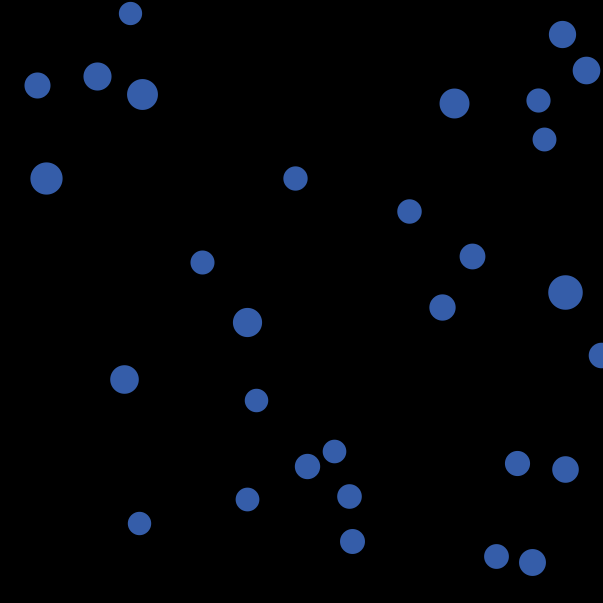
\includegraphics[width=0.4\textwidth]{figures/macrocoevol_example_virtual_0_t0}\hspace{0.2cm}
 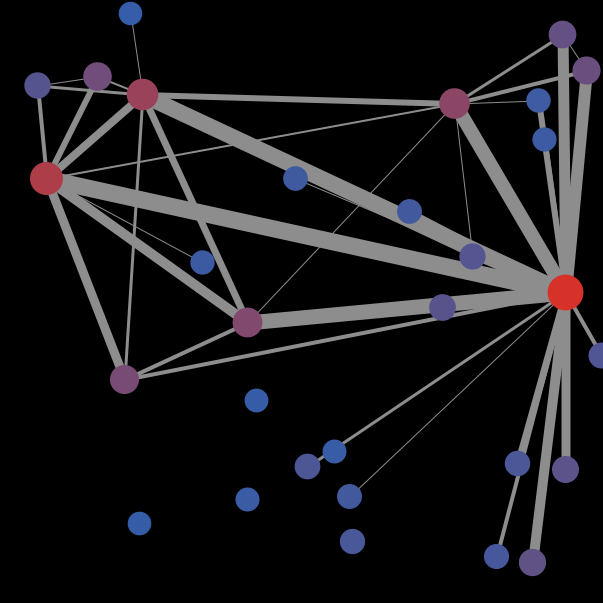
\includegraphics[width=0.4\textwidth]{figures/macrocoevol_example_virtual_0_tf}
 
 {\small\textit{Exemple of run ($t_f=30$). Level of red gives overall growth and link width flows.}}
 
}


\sframe{Synthetic system of cities}{

\justify

Generation of synthetic systems of cities for model exploration:

\medskip

\begin{itemize}
	\item Cities at random locations (farther from each other by a fixed radius $r_0 = 10$); population distribution with a scaling law $P_i = P_0\cdot i^{-\alpha_S}$ ($\alpha_S$ parameter, $P_0 = 100000$, for $N = 30$ cities)
	\item Create a grid network with nodes at a fixed distance $r_N = 15$; remove a fixed proportion $p_l = 0.2$ of links; jitter node positions by $\pm r_N$ for each coordinate (avoids ties in shortest routes and oscillating behaviors e.g.)
	\item Connect cities to the network with euclidian projection to closest link
\end{itemize}

\medskip

Applying the method of \cite{raimbault2018space} for spatial sensitivity to the SimpopNet model, \cite{raimbault2018unveiling} shows that the model is sensible to some (e.g. $\alpha_S$) $\rightarrow$ remains to be checked here.


% TODO : vraiment pas teste la sensiiblite au nombre de villes ; should be okay as indicators are integrated ? -> but possibly different qualitative regimes. (here N=30 reasonable for the "spatial extent" and size of cities : scaled european-type urban system ?)


}







%%%%%%%%%%%%%%%%%%%%%
\begin{frame}[allowframebreaks]
\frametitle{References}
\bibliographystyle{apalike}
\bibliography{biblio}
\end{frame}
%%%%%%%%%%%%%%%%%%%%%%%%%%%%










\end{document}







